\documentclass[13pt]{article}
\usepackage[utf8]{vietnam}
\usepackage[paperheight=29.7cm,paperwidth=21cm,right=2cm,left=3cm,top=2cm,bottom=2.5cm]{geometry}
\usepackage[table,xcdraw]{xcolor}
\usepackage{changepage}
\usepackage{indentfirst} % Thư viện thụt đầu dòng
\usepackage{graphicx}
\usepackage{subfig}
\usepackage{natbib}
\usepackage{color}
\usepackage{titlesec} 
\usepackage{amsmath}
\usepackage{amsfonts}
\usepackage{amssymb}
\usepackage{multirow}
\usepackage{indentfirst}
\usepackage{booktabs}
% Định dạng mục lục
\usepackage{tocloft}
\usepackage{tocloft}
\usepackage{url}
\usepackage{setspace} % Để điều chỉnh giãn dòng
\usepackage{times} % Sử dụng kiểu chữ Times New Roman
%\titlespacing*{\subsection}{0pt}{6pt}{0pt} % Heading 2
% Tùy chỉnh \section
\titleformat*{\section}{\centering\fontsize{16pt}{0pt}\selectfont\bfseries}
\titleformat*{\subsection}{\fontsize{16pt}{0pt}\selectfont \bfseries}
\renewcommand{\thesubsection}{\thesection.\arabic{subsection}} % Đặt lại số của subsection từ 1 mỗi section mới
\titleformat*{\subsubsection}{\fontsize{16pt}{0pt}\selectfont \bfseries }
\renewcommand{\baselinestretch}{1.4} % Giãn dòng 1.5
\setlength{\parskip}{0.3pt} % Spacing after
\setlength{\parindent}{1cm} % Set khoảng cách thụt đầu dòng mỗi đoạn
\setlength{\parskip}{1em}
\title{empty}
%\author{Nguyễn Thị Thu Hồng}
\usepackage{fancyhdr}
\pagenumbering{roman}
\pagestyle{fancy}
\fancyhf{} % Xóa các thiết lập mặc định
\fancyhead[C]{\thepage}
\renewcommand{\headrulewidth}{0pt} % Loại bỏ dòng gạch ngang dưới đầu trang
\renewcommand{\footrulewidth}{0pt}
\allowdisplaybreaks
\begin{document}
	\fontsize{14pt}{20pt}\selectfont
	\begin{center}
		TỔNG LIÊN ĐOÀN LAO ĐỘNG VIỆT NAM \\\textbf{TRƯỜNG ĐẠI HỌC TÔN ĐỨC THẮNG}\\
        \textbf{KHOA CÔNG NGHỆ THÔNG TIN}\\
		---------------------
	\end{center}
	%\maketitle
	\vspace{1cm}
	\begin{figure}[h]
		\centering
		\includegraphics[width=0.3\linewidth]{image/Logo.png}
	\end{figure}
	\vspace{-1cm}
	\vspace{1cm}
	\fontsize{20pt}{20pt}\selectfont
	\begin{center}
		\textbf{BÁO CÁO CUỐI KÌ}\\
        \textbf{MÔN THIẾT KẾ MẠNG}
	\end{center}
	\vspace{0.5cm}
	\fontsize{16pt}{20pt}\selectfont
	\begin{center}\Huge
		\textbf{Thiết kế hệ thống mạng VxLAN cho doanh nghiệp có hai chi nhánh}	
	\end{center}
    \vspace{0.5cm}
	\fontsize{16pt}{20pt}\selectfont
	\begin{flushright}\Large
		\textbf{\textbf{\textit{Người hướng dẫn: }\textbf{Giảng viên Lê Viết Thanh }}
        \\\textbf{\textit{Người thực hiện: }\textbf{Nguyễn Thị Thu Hồng - 52100962
        \\Nguyễn Đặng Trúc Duyên - 52100404}}\\
        \textbf{\textit{Lớp: }\textbf{21050401}}\\
        \textbf{\textit{Khoá: }\textbf{21}}
        }
	\end{flushright}
	\vspace{2cm}
	\fontsize{16pt}{20pt}\selectfont
	\begin{center}
		\textbf{THÀNH PHỐ HỒ CHÍ MINH, 2024}
	\end{center}

\newpage
	\fontsize{14pt}{20pt}\selectfont
	\begin{center}
		TỔNG LIÊN ĐOÀN LAO ĐỘNG VIỆT NAM \\\textbf{TRƯỜNG ĐẠI HỌC TÔN ĐỨC THẮNG}\\
        \textbf{KHOA CÔNG NGHỆ THÔNG TIN}\\
		---------------------
	\end{center}
	%\maketitle
	\vspace{1cm}
	\begin{figure}[h]
		\centering
		\includegraphics[width=0.3\linewidth]{image/Logo.png}
	\end{figure}
	\vspace{-1cm}
	\vspace{1cm}
	\fontsize{20pt}{20pt}\selectfont
	\begin{center}
		\textbf{BÁO CÁO CUỐI KÌ}\\
        \textbf{MÔN THIẾT KẾ MẠNG}
	\end{center}
	\vspace{0.5cm}
	\fontsize{16pt}{20pt}\selectfont
	\begin{center}\Huge
		\textbf{Thiết kế hệ thống mạng VxLAN cho doanh nghiệp có hai chi nhánh}	
	\end{center}
    \vspace{0.5cm}
	\fontsize{16pt}{20pt}\selectfont
	\begin{flushright}\Large
		\textbf{\textbf{\textit{Người hướng dẫn: }\textbf{Giảng viên Lê Viết Thanh }}
        \\\textbf{\textit{Người thực hiện: }\textbf{Nguyễn Thị Thu Hồng - 52100962
        \\Nguyễn Đặng Trúc Duyên - 52100404}}\\
        \textbf{\textit{Lớp: }\textbf{21050401}}\\
        \textbf{\textit{Khoá: }\textbf{21}}
        }
	\end{flushright}
	\vspace{2cm}
	\fontsize{16pt}{20pt}\selectfont
	\begin{center}
		\textbf{THÀNH PHỐ HỒ CHÍ MINH, 2024}
	\end{center}
    
\renewcommand\thesection{\arabic{section}}


\pagenumbering{arabic}
\pagestyle{fancy}
\fancyhf{}
\fancyhead[C]{\thepage}
\renewcommand{\headrulewidth}{0pt} % Loại bỏ dòng gạch ngang dưới đầu trang

\lhead{\textbf{Báo cáo cuối kỳ}}
\chead{}
\rhead{\textbf{{Thiết kế mạng}}}
\lfoot{\textbf{Giảng viên: Lê Viết Thanh}}
\cfoot{}
\rfoot{\thepage}

\newpage
\section*{LỜI CẢM ƠN}
\addcontentsline{toc}{section}{LỜI CẢM ƠN} % Thêm vào mục lục
    Em xin gửi lời cảm ơn chân thành đến Ban Giám Hiệu trường Đại học Tôn Đức Thắng đã tạo điều kiện uận lợi cho em trong suốt quá trình học tập và nghiên cứu.
    
    Em xin chân thành cảm ơn Khoa Công Nghệ Thông Tin đã cung cấp môi trường học tập và nghiên cứu uyên nghiệp, giúp em có thể tiếp thu và áp dụng những kiến thức quý báu vào thực tiễn. Đặc biệt, em xin bày lòng biết ơn sâu sắc đến thầy Lê Viết Thanh, người đã tận tâm hướng dẫn và đồng hành cùng em trong suốt á trình thực hiện đồ án này. Những chỉ dẫn và góp ý của thầy đã giúp em hoàn thiện đề tài một cách tốt nhất.
    
    Cuối cùng, em xin kính chúc quý Thầy Cô trong Khoa Công Nghệ Thông Tin luôn dồi dào sức khỏe, tràn y niềm tin và nhiệt huyết để tiếp tục sứ mệnh cao đẹp của mình là truyền đạt kiến thức cho thế hệ mai sau.
\newpage

\section*{ĐỒ ÁN ĐƯỢC HOÀN THÀNH TẠI TRƯỜNG ĐẠI HỌC TÔN ĐỨC THẮNG}
    Tôi xin cam đoan đây là sản phẩm đồ án của riêng chúng tôi và được sự hướng dẫn của ThS Lê Viết Thanh. Các nội dung nghiên cứu, kết quả trong đề tài này là trung thực và chưa công bố dưới bất kỳ hình thức nào trước đây. Những số liệu trong các bảng biểu phục vụ cho việc phân tích, nhận xét, đánh giá được chính tác giả thu thập từ các nguồn khác nhau có ghi rõ trong phần tài liệu tham khảo.
    
    Ngoài ra, trong đồ án còn sử dụng một số nhận xét, đánh giá cũng như số liệu của các tác giả khác, cơ quan tổ chức khác đều có trích dẫn và chú thích nguồn gốc.
    
    Nếu phát hiện có bất kỳ sự gian lận nào tôi xin hoàn toàn chịu trách nhiệm về nội dung đồ án của mình. Trường đại học Tôn Đức Thắng không liên quan đến những vi phạm tác quyền, bản quyền do tôi gây ra trong quá trình thực hiện (nếu có).

\begin{flushright}
    \textit{TP. Hồ Chí Minh, ngày 01 tháng 12 năm 2024}\\      
    \begin{adjustwidth}{10cm}{}
    \textit{Tác giả}\\
    \end{adjustwidth} 
    
    \begin{adjustwidth}{8cm}{}
	\textit{(ký tên và ghi rõ họ tên)}\\
    \end{adjustwidth} 
    
    \begin{adjustwidth}{8.5cm}{}
    \textit{Nguyễn Thị Thu Hồng}\\
    \end{adjustwidth} 
    
    \begin{adjustwidth}{8cm}{}
    \textit{Nguyễn Đặng Trúc Duyên}
    \end{adjustwidth} 
\end{flushright}


\newpage
\section*{PHẦN XÁC NHẬN VÀ ĐÁNH GIÁ CỦA GIẢNG VIÊN}
\addcontentsline{toc}{section}{PHẦN XÁC NHẬN VÀ ĐÁNH GIÁ CỦA GIẢNG VIÊN} % Thêm vào mục lục
Phần xác nhận của GV hướng dẫn\\
\vspace{3cm}
\begin{flushright}
    Tp. Hồ Chí Minh, ngày     tháng   năm   \\
	\begin{adjustwidth}{10cm}{}
	(kí và ghi họ tên)\\
    \end{adjustwidth}
    
\end{flushright}

    
Phần đánh giá của GV chấm bài\\
\vspace{3cm}
\begin{flushright}
    Tp. Hồ Chí Minh, ngày     tháng   năm   \\
    \begin{adjustwidth}{10cm}{}
	(kí và ghi họ tên)\\
    \end{adjustwidth}
    
\end{flushright}


\newpage

\section*{TÓM TẮT}
\addcontentsline{toc}{section}{TÓM TẮT} % Thêm vào mục lục
Trong bối cảnh số hóa và nhu cầu kết nối ngày càng cao, các doanh nghiệp vừa và nhỏ (SME) phải đối mặt với thách thức nâng cấp hạ tầng công nghệ thông tin để đáp ứng yêu cầu kinh doanh phức tạp. Giải pháp sử dụng VXLAN kết hợp mô hình mạng 2-Tier (Spine-Leaf) là lựa chọn lý tưởng để tối ưu hóa hiệu suất, giảm thiểu chi phí và mở rộng mạng linh hoạt. VXLAN vượt qua giới hạn của VLAN truyền thống, tận dụng hạ tầng Layer 3 để cải thiện hiệu quả mạng, trong khi mô hình 2-Tier giúp giảm độ trễ và tối ưu băng thông. Giải pháp này cũng đảm bảo bảo mật thông tin và hỗ trợ các công nghệ mới như Cloud Computing, IoT và Big Data, phù hợp với chiến lược chuyển đổi số của doanh nghiệp. Đề tài này không chỉ mang tính lý thuyết mà còn có tính ứng dụng cao, giúp các doanh nghiệp vừa và nhỏ nâng cao hiệu quả hoạt động, tối ưu hóa tài nguyên và chuẩn bị cho tương lai phát triển bền vững.

\newpage
\addcontentsline{toc}{section}{MỤC LỤC} % Thêm vào mục lục
\tableofcontents
\newpage

\section*{DANH MỤC KÍ HIỆU VÀ CHỮ VIẾT TẮT}
\addcontentsline{toc}{section}{DANH MỤC KÍ HIỆU VÀ CHỮ VIẾT TẮT} % Thêm vào mục lục

\textbf{CÁC KÝ HIỆU}\\

\textbf{CÁC CHỮ VIẾT TÁT}\\
SME - Small and Medium Enterprise\\
PAN - Personal Area Network\\
LAN - Local Area Network\\
CAN - Campus Area Network\\
MAN - Metropolitan Area Network\\
WAN - Wide Area Network\\
DHCP - Dynamic Host Configuration Proto-
col\\
DNS - Domain Name System\\
FTP - File Transfer Protocol\\
VLAN - Virtual Local Area Network\\
VXLAN - Virtual Extensible LAN\\
MAC - Media Access Control Address\\
UDP - User Datagram Protocol\\
DMZ -Demilitarized Zone
\newpage

\section*{DANH MỤC CÁC BẢNG BIỂU, HÌNH VẼ, ĐỒ THỊ}
\addcontentsline{toc}{section}{DANH MỤC CÁC BẢNG BIỂU, HÌNH VẼ, ĐỒ THỊ} % Thêm vào mục lục
\textbf{DANH MỤC HÌNH}\\
\renewcommand{\listfigurename}{}
\listoffigures

\newpage
\textbf{DANH MỤC BẢNG}\\
\renewcommand{\listtablename}{}
\listoftables

\newpage

\setcounter{section}{1} % Đặt số thứ tự cho section
\section*{CHƯƠNG 1 - TỔNG QUAN ĐỀ TÀI}
\addcontentsline{toc}{section}{CHƯƠNG 1 - TỔNG QUAN ĐỀ TÀI}
    \subsection{Lý do chọn đề tài}
        Trong thời đại số hóa hiện nay, các doanh nghiệp vừa và nhỏ (SME) đang đứng trước áp lực phải nâng cấp hạ tầng công nghệ thông tin để đáp ứng nhu cầu kinh doanh ngày càng phức tạp. Với sự phát triển mạnh mẽ của các ứng dụng đòi hỏi khả năng xử lý nhanh chóng và liên tục, cùng với xu hướng làm việc từ xa và kết nối chi nhánh, việc xây dựng một mạng lưới linh hoạt, hiệu quả và an toàn đã trở thành một yếu tố cốt lõi trong chiến lược phát triển của các doanh nghiệp này. Tuy nhiên, một bài toán khó đặt ra là làm thế nào để cân bằng giữa hiệu suất cao và tối ưu chi phí trong điều kiện nguồn lực tài chính hạn chế.

        Trong bối cảnh đó, giải pháp sử dụng VXLAN (Virtual Extensible LAN) và mô hình 2-Tier (Spine-Leaf) được xem là một lựa chọn lý tưởng để thiết kế mạng cho các doanh nghiệp vừa và nhỏ. VXLAN mang đến khả năng mở rộng không gian mạng vượt xa giới hạn VLAN truyền thống, đáp ứng tốt nhu cầu phát triển dài hạn của doanh nghiệp. Đồng thời, công nghệ này tận dụng tối đa hạ tầng Layer 3, giúp cải thiện hiệu suất và giảm thiểu sự phụ thuộc vào mạng Layer 2, vốn dễ gặp vấn đề khi mở rộng quy mô. Bên cạnh đó, mô hình 2-Tier với kiến trúc Spine-Leaf mang lại hiệu quả vượt trội nhờ khả năng giảm độ trễ, tối ưu hóa băng thông và hỗ trợ mở rộng linh hoạt mà không làm gián đoạn hệ thống hiện có.

        Việc ứng dụng VXLAN kết hợp mô hình 2-Tier không chỉ giải quyết các thách thức về mở rộng mạng mà còn đảm bảo bảo mật thông tin trong bối cảnh các mối đe dọa an ninh mạng ngày càng phức tạp. Khả năng phân chia và cô lập lưu lượng giữa các VLAN giúp doanh nghiệp quản lý dữ liệu tốt hơn, đặc biệt là trong các phòng ban quan trọng như tài chính, nhân sự hay chi nhánh từ xa. Hơn nữa, kiến trúc mạng này còn phù hợp với các doanh nghiệp đang trong quá trình chuyển đổi số, sẵn sàng hỗ trợ các công nghệ hiện đại như Cloud Computing, IoT và Big Data.

        Với những lợi ích trên, đề tài "Thiết kế mạng cho doanh nghiệp vừa và nhỏ, sử dụng VXLAN và mô hình 2-Tier" không chỉ mang ý nghĩa nghiên cứu mà còn có tính ứng dụng thực tiễn cao. Đây là giải pháp mang lại giá trị lâu dài, giúp doanh nghiệp vừa và nhỏ nâng cao hiệu quả hoạt động, tối ưu nguồn lực và sẵn sàng thích nghi với những thay đổi trong tương lai.
        
    \subsection{Mục tiêu}
    \subsubsection{Mục tiêu tổng quát}
    \begin{itemize}
        \item Thiết kế một hệ thống mạng hiệu quả, linh hoạt và dễ mở rộng, đáp ứng nhu cầu hiện tại và tương lai của doanh nghiệp vừa và nhỏ, đồng thời đảm bảo khả năng bảo mật và hiệu suất hoạt động cao.
        \item Đề xuất giải pháp sử dụng VXLAN và mô hình 2-Tier để khắc phục những hạn chế của các kiến trúc mạng truyền thống, tối ưu hóa việc sử dụng tài nguyên mạng.
    \end{itemize}

    \subsubsection{Mục tiêu cụ thể}
    \begin{enumerate}
        \item \textbf{Phân tích và đánh giá yêu cầu hệ thống mạng}
        \begin{itemize}
            \item Xác định các yêu cầu thực tế của doanh nghiệp vừa và nhỏ, bao gồm:
            \begin{itemize}
                \item Khả năng mở rộng mạng.
                \item Hiệu năng xử lý và băng thông.
                \item Tính bảo mật và cô lập dữ liệu.
                \item Tối ưu chi phí và tài nguyên mạng.
            \end{itemize}
        \end{itemize}
        
        \item \textbf{Đề xuất giải pháp công nghệ}
        \begin{itemize}
            \item Giải thích chi tiết về công nghệ VXLAN, bao gồm cơ chế hoạt động và lợi ích trong việc mở rộng mạng.
            \item Mô tả kiến trúc mô hình 2-Tier (Spine-Leaf), các thành phần chính và cách thức hoạt động để tối ưu băng thông và giảm độ trễ.
        \end{itemize}

        \item \textbf{Thiết kế hệ thống mạng}
        \begin{itemize}
            \item Xây dựng sơ đồ mạng với sự kết hợp của VXLAN và mô hình 2-Tier, bao gồm:
            \begin{itemize}
                \item Cách phân chia VLAN và kết nối giữa các tầng mạng.
                \item Cách cấu hình các thành phần chính như switch Spine, switch Leaf, và các thiết bị kết nối.
                \item Cơ chế định tuyến, cân bằng tải và dự phòng để đảm bảo hoạt động liên tục.
            \end{itemize}
        \end{itemize}

        \item \textbf{Phân tích hiệu năng và băng thông}
        \begin{itemize}
            \item Tính toán và đánh giá khả năng đáp ứng về hiệu năng mạng (băng thông, độ trễ, dung lượng xử lý).
            \item Đề xuất các cơ chế quản lý băng thông và lưu lượng mạng giữa các phòng ban hoặc chi nhánh.
        \end{itemize}

        \item \textbf{Đề xuất giải pháp bảo mật}
        \begin{itemize}
            \item Tích hợp các công nghệ bảo mật như tường lửa, VPN, và Access Control List (ACL) vào kiến trúc mạng.
            \item Đề xuất cách sử dụng VXLAN để cô lập lưu lượng giữa các bộ phận, phòng ban và chi nhánh, bảo vệ dữ liệu quan trọng.
        \end{itemize}

        \item \textbf{Đánh giá chi phí triển khai và vận hành}
        \begin{itemize}
            \item Ước tính chi phí triển khai mạng dựa trên mô hình đề xuất.
            \item So sánh giữa chi phí đầu tư ban đầu và lợi ích dài hạn (hiệu năng, mở rộng, tiết kiệm chi phí vận hành).
        \end{itemize}

        \item \textbf{Xây dựng kịch bản mở rộng trong tương lai}
        \begin{itemize}
            \item Thiết kế các phương án mở rộng khi doanh nghiệp phát triển thêm chi nhánh hoặc tăng quy mô nhân sự.
            \item Đề xuất các giải pháp để nâng cấp hệ thống mà không gây gián đoạn hoạt động.
        \end{itemize}
    
    \end{enumerate}

    \subsubsection{Kết quả kỳ vọng}
    Hoàn thiện một báo cáo chi tiết về thiết kế mạng dựa trên VXLAN và mô hình 2-Tier, phù hợp với yêu cầu của doanh nghiệp vừa và nhỏ.
    
    Cung cấp một giải pháp thực tế, có thể triển khai hiệu quả, đồng thời đáp ứng nhu cầu phát triển trong tương lai của doanh nghiệp.
    
    Góp phần tối ưu hóa chi phí đầu tư vào hạ tầng mạng, nâng cao hiệu suất hoạt động và khả năng cạnh tranh của doanh nghiệp.

    \subsection{Đối tượng và phạm vi nghiên cứu}
    \subsubsection{Đối tượng nghiên cứu}
    \begin{enumerate}
        \item \textbf {Doanh nghiệp vừa và nhỏ (SME)}\\
        Tập trung vào các doanh nghiệp có quy mô nhân sự từ 50 đến 500 người, với yêu cầu về hệ thống mạng vừa phải nhưng cần đảm bảo hiệu suất, tính ổn định và khả năng mở rộng.

        \item \textbf{Hạ tầng mạng}\\
        Bao gồm các thành phần chính như switch, router, máy chủ, các thiết bị đầu cuối (máy tính, thiết bị IoT), và các giao thức mạng liên quan.

        \item \textbf{Công nghệ VXLAN}\\
        Là giải pháp chính để mở rộng mạng Layer 2 qua hạ tầng Layer 3, giúp khắc phục các hạn chế của VLAN truyền thống

        \item \textbf{Mô hình 2-Tier (Spine-Leaf)}\\
        Một kiến trúc mạng hiện đại với hai lớp chính (Spine và Leaf), tối ưu hóa cho các doanh nghiệp có quy mô vừa và nhỏ.

        \item \textbf{Các vấn đề bảo mật và quản lý mạng}\\
        Bao gồm cách cô lập lưu lượng, bảo vệ dữ liệu, và quản lý lưu lượng giữa các phòng ban hoặc chi nhánh.

    \end{enumerate}
    
    \subsubsection{Phạm vi nghiên cứu}
\begin{enumerate}
        \item \textbf{Phạm vi không gian}
    \begin{itemize}
        \item Tập trung nghiên cứu và thiết kế hạ tầng mạng cho các doanh nghiệp vừa và nhỏ hoạt động trong các lĩnh vực như tài chính, thương mại, sản xuất, hoặc dịch vụ.
        \item Mô hình mạng được thiết kế bao gồm:
        \begin{itemize}
            \item Trụ sở chính: Là trung tâm quản lý dữ liệu, với yêu cầu băng thông cao và khả năng mở rộng tốt.
            \item Chi nhánh: Kết nối từ xa qua mạng WAN/VPN với trụ sở chính, yêu cầu kết nối ổn định và bảo mật.
            \item Khu vực DMZ:
            \begin{itemize}
                \item Là khu vực được cô lập giữa mạng nội bộ và mạng bên ngoài, chứa các máy chủ quan trọng như:
                \begin{itemize}
                    \item  Máy chủ ứng dụng: Đáp ứng yêu cầu truy cập từ bên ngoài (web server, email server, v.v.).
                    \item Máy chủ lưu trữ: Dành cho dữ liệu dùng chung hoặc phục vụ ứng dụng.
                    \item Máy chủ giám sát: Dùng để theo dõi trạng thái hệ thống và phát hiện các mối đe dọa.
                \end{itemize}
                \item Phân tích cơ chế bảo mật và cách cấu hình các thiết bị trong DMZ như firewall, router, và các chính sách Access Control.
            \end{itemize}
        \end{itemize}
    \end{itemize}

    \item \textbf{Phạm vi công nghệ}
    \begin{itemize}
        \item VXLAN: Nghiên cứu chi tiết cách thức hoạt động của giao thức này, bao gồm encapsulation, định tuyến overlay, và các lợi ích trong việc mở rộng không gian mạng.
        \item Kiến trúc Spine-Leaf (2-Tier):
        \begin{itemize}
            \item Cách thiết kế kết nối giữa các thiết bị Spine và Leaf để tối ưu hóa băng thông và giảm độ trễ.
            \item So sánh với mô hình 3-Tier để đánh giá ưu điểm trong hiệu năng và chi phí.
        \end{itemize}
        \item Bảo mật mạng:
        \begin{itemize}
            \item Tích hợp các cơ chế bảo mật như Access Control List (ACL), tường lửa, VPN, và phân chia VLAN cô lập giữa các phòng ban, chi nhánh, và DMZ.
            \item Sử dụng các chính sách bảo mật để ngăn chặn truy cập trái phép vào mạng nội bộ từ khu vực DMZ.
        \end{itemize}
    \end{itemize}

    \item \textbf{Phạm vi thời gian}
    \begin{itemize}
        \item Thiết kế mạng được thực hiện trong bối cảnh hiện nay, hướng tới các doanh nghiệp đang trong quá trình chuyển đổi số và mở rộng quy mô.
        \item Đề xuất giải pháp đáp ứng nhu cầu hiện tại và có thể mở rộng thêm trong khoảng 3-5 năm tới.
    \end{itemize}

    \item \textbf{Phạm vi ứng dụng}
    \begin{itemize}
        \item Tập trung vào các doanh nghiệp vừa và nhỏ, không đi sâu vào hệ thống phức tạp của doanh nghiệp lớn hoặc tổ chức viễn thông.
        \item Hướng đến các ngành nghề phổ biến như tài chính, sản xuất, thương mại, và dịch vụ, nơi yêu cầu hạ tầng mạng ổn định và bảo mật là ưu tiên.
        \item Giới hạn việc nghiên cứu vào các công nghệ và thiết bị phổ biến trên thị trường, đảm bảo tính khả thi và phù hợp với ngân sách của doanh nghiệp SME.
    \end{itemize}
\end{enumerate}

    \subsection{Phương pháp nghiên cứu}
    \begin{enumerate}
        \item \textbf{Phương pháp nghiên cứu lý thuyết}
        \begin{itemize}
            \item Thu thập tài liệu và tài nguyên học thuật:
            \begin{itemize}
                \item Tìm hiểu các tài liệu chuyên môn, sách, bài báo khoa học liên quan đến công nghệ VXLAN, mô hình Spine-Leaf (2-Tier), và các giải pháp bảo mật mạng.
                \item Khai thác tài nguyên từ các nguồn đáng tin cậy như IEEE, Cisco, Juniper, và các diễn đàn công nghệ mạng.
            \end{itemize}
            \item Phân tích và tổng hợp:
            \begin{itemize}
                \item Phân tích các khái niệm và nguyên tắc hoạt động của VXLAN, mô hình Spine-Leaf, và khu vực DMZ.
                \item Tổng hợp các ưu điểm và nhược điểm của các công nghệ được lựa chọn, so sánh với các giải pháp truyền thống để làm rõ tính hiệu quả.
            \end{itemize}
        \end{itemize}

        \item \textbf{Phương pháp nghiên cứu thực nghiệm}
        \begin{itemize}
            \item Thiết kế mô hình mạng:
            \begin{itemize}
                \item Xây dựng một mô hình mạng doanh nghiệp dựa trên công nghệ VXLAN và kiến trúc Spine-Leaf.
                \item Thiết kế bao gồm phân chia VLAN, cấu hình DMZ, kết nối VPN giữa trụ sở chính và chi nhánh, và triển khai các cơ chế bảo mật.
            \end{itemize}
            \item Mô phỏng hệ thống:
            \begin{itemize}
                \item Sử dụng các công cụ mô phỏng mạng như Cisco Packet Tracer hoặc EVE-NG để kiểm tra hoạt động của hệ thống.
                \item Mô phỏng các tình huống thực tế, chẳng hạn như:
                \begin{itemize}
                    \item Lưu lượng truy cập từ các phòng ban trong nội bộ.
                    \item Lưu lượng từ mạng bên ngoài truy cập khu vực DMZ.
                    \item Kết nối VPN giữa các chi nhánh và trụ sở chính.
                \end{itemize}
            \end{itemize}
            \item Đánh giá hiệu năng:
            \begin{itemize}
                \item Đo lường băng thông, độ trễ, và hiệu suất xử lý của mô hình mạng trong các kịch bản khác nhau.
                \item Kiểm tra khả năng mở rộng của hệ thống khi tăng lưu lượng hoặc bổ sung thiết bị.
            \end{itemize}
        \end{itemize}

        \item \textbf{Phương pháp đánh giá và cải tiến}
        \begin{itemize}
            \item Đánh giá kết quả của mô hình đề xuất qua các tiêu chí: hiệu năng, chi phí, bảo mật, và khả năng mở rộng.
            \item Tiến hành cải tiến mô hình nếu phát hiện các hạn chế hoặc khả năng tối ưu hóa trong quá trình kiểm thử.
        \end{itemize}
    \end{enumerate}

    \subsection{Ý nghĩa lý luận và thực tiễn}
    \subsubsection{Ý nghĩa lý luận}
    \begin{enumerate}
        \item \textbf{Đóng góp vào lĩnh vực công nghệ mạng:}
            \begin{itemize}
                \item Nghiên cứu cung cấp một cách nhìn tổng quát về việc ứng dụng công nghệ VXLAN trong việc mở rộng mạng Layer 2 và cải thiện khả năng quản lý so với VLAN truyền thống.
                \item Xác định và phân tích ưu điểm của mô hình 2-Tier (Spine-Leaf) trong việc giảm độ phức tạp, tăng hiệu suất, và khả năng mở rộng của hạ tầng mạng.
                \item Bổ sung vào kho tài liệu lý thuyết về kiến trúc mạng, đặc biệt là cho các doanh nghiệp vừa và nhỏ (SME), đối tượng ít được nghiên cứu sâu so với doanh nghiệp lớn.
            \end{itemize}
            
        \item \textbf{Đề xuất giải pháp bảo mật và quản lý:}
            \begin{itemize}
                \item Đưa ra cơ sở lý luận cho việc triển khai các khu vực bảo mật như DMZ, VLAN cô lập, và các chính sách bảo mật khác nhằm bảo vệ tài nguyên doanh nghiệp trước các mối đe dọa từ bên ngoài.
                \item Khẳng định vai trò của các công nghệ hiện đại như VXLAN và kiến trúc Spine-Leaf trong việc đối phó với các thách thức về băng thông, hiệu năng, và bảo mật.
            \end{itemize}
    \end{enumerate}

    \subsubsection{Ý nghĩa thực tiễn}
    \begin{enumerate}
        \item \textbf{Ứng dụng vào triển khai thực tế:}
            \begin{itemize}
                \item Đề tài cung cấp một thiết kế mạng mẫu có thể áp dụng trực tiếp cho các doanh nghiệp vừa và nhỏ, đảm bảo hiệu suất cao, bảo mật và khả năng mở rộng.Giúp doanh nghiệp SME tối ưu hóa chi phí đầu tư và vận hành hệ thống mạng mà vẫn đáp ứng được nhu cầu ngày càng tăng về dữ liệu và kết nối.
                \item 
            \end{itemize}
        \item \textbf{Hỗ trợ chuyển đổi số:}
            \begin{itemize}
                \item Giải pháp mạng này phù hợp với xu hướng chuyển đổi số, hỗ trợ doanh nghiệp ứng dụng các công nghệ mới như Cloud Computing, IoT, và Big Data một cách hiệu quả.
                \item Góp phần vào việc hiện đại hóa hạ tầng công nghệ thông tin của doanh nghiệp, tăng cường khả năng cạnh tranh trong thị trường số hóa.
            \end{itemize}
        \item \textbf{Định hướng phát triển bền vững:}
            \begin{itemize}
                \item Đề tài xây dựng một mô hình mạng có khả năng mở rộng linh hoạt, giúp doanh nghiệp phát triển bền vững trong tương lai mà không cần tái cấu trúc lớn về hạ tầng.
                \item Giảm thiểu rủi ro về bảo mật và hiệu suất mạng, hỗ trợ doanh nghiệp đáp ứng các thách thức trong môi trường kinh doanh hiện đại.
            \end{itemize}
        \item \textbf{Làm tài liệu tham khảo:}
            \begin{itemize}
                \item Có thể sử dụng làm tài liệu tham khảo cho các sinh viên công nghệ thông tin, hoặc những người đang tìm kiếm giải pháp tối ưu hóa mạng cho doanh nghiệp vừa và nhỏ.
            \end{itemize}
    \end{enumerate}

    \subsection{Cấu trúc bài báo cáo}
    Bài báo cáo gồm 4 chương:
    \begin{enumerate}
        \item \textbf{Chương 1: Tổng quan đề tài}
        \begin{itemize}
            \item Giới thiệu sơ lược, tổng quan về đề tài, mục tiêu của đề tài.
        \end{itemize}
        
        \item \textbf{Chương 2: Cở sở lý thuyết}
        \begin{itemize}
            \item Tìm hiểu và nghiên cứu các kiến thức về mạng LAN, kỹ thuật xây dựng VXLAN và triển khai mô hình 2-Tier cho hệ thống.
            \item Giới thiệu cơ sở lý thuyết cần có để thực hiện đề tài và các lý thuyết liên quan đến đề tài
        \end{itemize}
        \item \textbf{Chương 3: Phân tích và thiết kế hệ thống}
        \begin{itemize}
            \item Khảo sát, phân tích thông tin về khu vực thực hiện đề tài.
            \item Trình bày định hướng thiết kế hệ thống.
            \item Thiết kế các sơ đồ mô phỏng mô hình mạng.
            \item Liệt kê các thông tin cấu hình hệ thống.
        \end{itemize}
        \item \textbf{Chương 4: Tổng kết}
        \begin{itemize}
            \item Trình bày các kết quả đạt được sau khi hoàn thành
            \item Trình bày hướng phát triển dự án trong tương lai.
        \end{itemize}
    \end{enumerate}

\newpage
% Chương 2  
\renewcommand{\thesubsection}{\thesection.\arabic{subsection}} % Đặt lại số của subsection từ 1 mỗi section mới
\setcounter{section}{2} % Đặt số thứ tự cho section
\setcounter{subsection}{0}
\section*{CHƯƠNG 2 - TỔNG QUAN LÝ THUYẾT}
\addcontentsline{toc}{section}{CHƯƠNG 2 - CƠ SỞ LÝ THUYẾT}
\subsection{Tổng quan Mạng máy tính}
\subsubsection{Mạng máy tính là gì?}
\begin{itemize}
    \item Mạng máy tính là một kênh truyền thông tin dùng cho chúng ta có thể chia sẻ dữ liệu với các máy tính hoặc thiết bị khác kết nối với cùng một mạng. Nó còn được gọi là Mạng Dữ liệu.
    \item Các tiêu chí về mạng máy tính :khả năng hoạt động, độ tin cậy, độ bảo mật, khả năng mở rộng, ...
\end{itemize}
\subsubsection{Các loại hình mạng máy tính:}
\begin{figure}[h!]
        \centering
        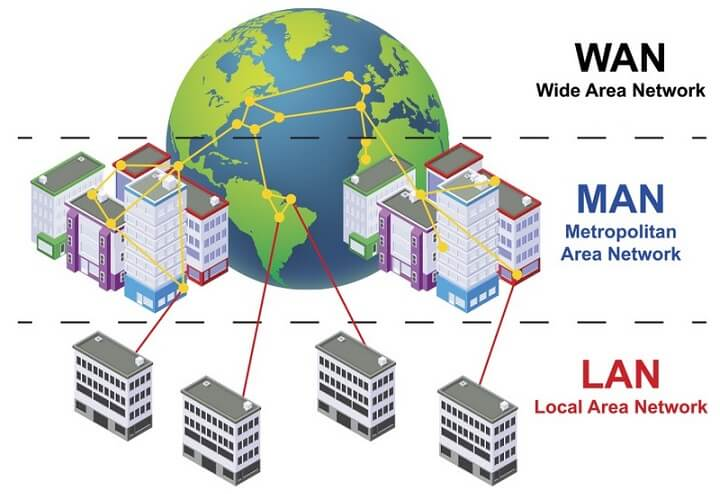
\includegraphics[width=0.7\linewidth]{image/image5.png}
            \caption{Các loại hình mạng máy tính}
            \label{fig:label1}
    \end{figure}
\begin{enumerate}

    \item \textbf{Personal Area Network (PAN):}
    \begin{figure}[h!]
        \centering
        \includegraphics[width=0.7\linewidth]{image/image0.png}
            \caption{Personal Area Network (PAN)}
            \label{fig:label1}
    \end{figure}

    \begin{itemize}
        \item Các thiết bị kết nối với nhau trong phạm vi của một cá nhân, thường trong phạm vi 10 mét.
        \item Ví dụ, một mạng không dây kết nối máy tính với bàn phím, chuột hoặc máy in là PAN.
        \item Ngoài ra, các thiết bị kĩ thuật số cá nhân điều khiển máy trợ thính hoặc máy điều hòa nhịp tim của người dùng phù hợp với PAN. Một ví dụ khác của PAN là Bluetooth. Thông thường, loại mạng này cũng có thể được kết nối với nhau mà không cần dây nối với Internet hoặc các mạng khác.
    \end{itemize}
    
    \item \textbf{Local Area Network (LAN):}
    \begin{figure}[h!]
        \centering
        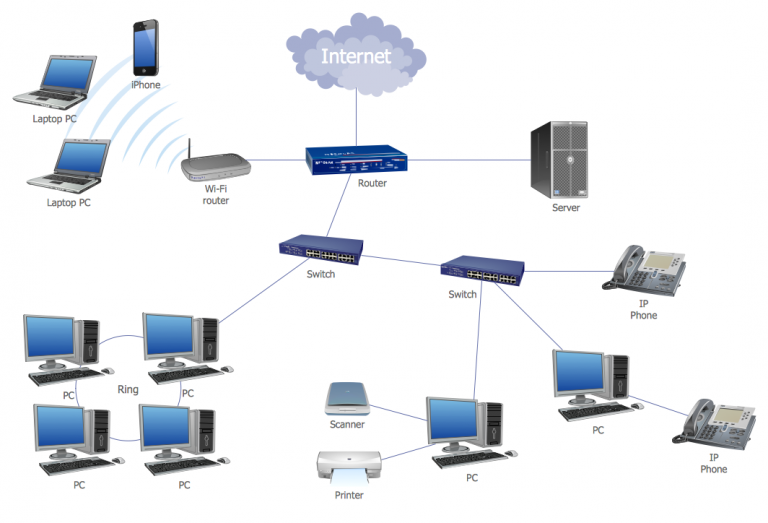
\includegraphics[width=0.7\linewidth]{image/image1.png}
            \caption{Local Area Network (LAN)}
            \label{fig:label1}
    \end{figure}
    \begin{itemize}
        \item Mạng cho cá nhân với một khu vực địa lý nhỏ, chẳng hạn như nhà, văn phòng, tòa nhà hoặc nhóm các tòa nhà (ví dụ: trường học,bệnh viện,…). 
        \item Có hai loại mạng LAN chính: LAN có dây và LAN không dây. Một số đặc điểm cơ bản của mạng cục bộ bao gồm:
        \begin{itemize}
            \item Quy mô mạng nhỏ: Phạm vi hoạt động của mạng LAN thường giới hạn trong vài km, kết nối các máy tính trong cùng một tòa nhà hoặc doanh nghiệp. Quá trình quản lý và bảo trì mạng cũng đơn giản hơn so với các loại mạng khác.
            \item Công nghệ truyền dẫn: Mạng LAN thường sử dụng công nghệ quảng bá, với một cáp đơn kết nối tất cả các máy tính. Tốc độ truyền dữ liệu rất cao, từ 10 đến 100 Mbps, thậm chí có thể đạt tới hàng trăm Gbps, với thời gian trễ rất thấp (khoảng 10 µs) và độ tin cậy cao, tỷ lệ lỗi bit dao động từ 10\textsuperscript{-8} đến 10\textsuperscript{-11}.
        \end{itemize}
    \end{itemize}

    \item \textbf{Campus Area Network (CAN):}  
    \begin{figure}[h!]
        \centering
        \includegraphics[width=0.7\linewidth]{image/image2.png}
            \caption{Campus Area Network (CAN)}
            \label{fig:label1}
    \end{figure}
    \begin{itemize}
        \item Đôi khi một mạng LAN cần kết nối mạng từ một số tòa nhà như trường học, bệnh viện, ... Loại mạng LAN lớn nhất này dựa vào các mạng đường trục mạnh mẽ (thường là cáp quang) để cho phép các tòa nhà này được kiểm soát bởi một quản trị viên mạng LAN duy nhất. Nếu khuôn viên nằm ở một vị trí địa lý duy nhất được kết nối bằng Ethernet, thì đó là mạng LAN. Tuy nhiên, nếu khoảng cách đủ lớn khiến chi phí cáp mạng tự quản lý cao hơn, các doanh nghiệp lớn hơn sẽ dựa vào một bộ giao thức mới do nhà cung cấp dịch vụ quản lý. Đây là nơi chúng ta chuyển từ mạng LAN sang mạng WAN. CAN là loại mạng duy nhất có thể là mạng LAN hoặc WAN tùy thuộc vào các giao thức được sử dụng để kết nối các tòa nhà khác nhau.
    \end{itemize}
    
    \item \textbf{Metropolitan Area Network (MAN):}
    \begin{figure}[h!]
        \centering
        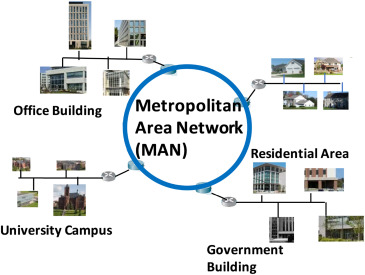
\includegraphics[width=0.7\linewidth]{image/image3.png}
            \caption{Metropolitan Area Network (MAN)}
            \label{fig:label1}
    \end{figure}
    
    \begin{itemize}
        \item Phạm vi hoạt động lớn hơn mạng LAN, từ nhiều khối nhà đến toàn bộ thành phố. Khả năng truyền dữ liệu từ vừa đến cao phụ thuộc vào kênh truyền thông của MAN. Một MAN có thể được sở hữu và điều hành bởi một tổ chức duy nhất, nhưng nó thường được sử dụng bởi nhiều cá nhân và tổ chức. MAN cũng có thể được sở hữu và vận hành như là các tiện ích công cộng. Họ thường cung cấp phương tiện cho việc kết nối mạng LAN. MAN có thể kéo dài đến 50km, các thiết bị được sử dụng là modem và dây/ cáp.
    \end{itemize}

    \item \textbf{Wide Area Network (WAN):}
    \begin{figure}[h!]
        \centering
        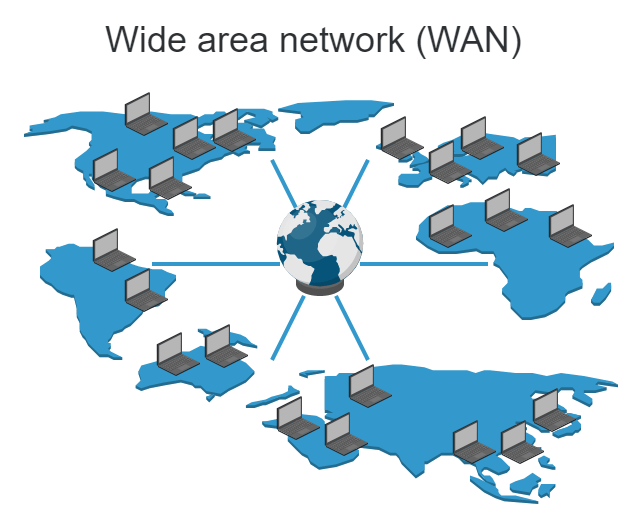
\includegraphics[width=0.7\linewidth]{image/image4.png}
            \caption{Wide Area Network (WAN)}
            \label{fig:label1}
    \end{figure}
    \begin{itemize}
        \item Phạm vi mạng mở rộng trên một khoảng cách địa lý rộng lớn. Mạng diện rộng được thiết lập với các mạng viễn thông thuê. Các doanh nghiệp, giáo dục và các cơ quan chính phủ sử dụng mạng diện rộng để chuyển tiếp dữ liệu cho nhân viên, sinh viên, khách hàng, người mua và nhà cung cấp từ các địa điểm khác nhau trên thế giới.
        \item Về bản chất, phương thức viễn thông này cho phép doanh nghiệp thực hiện hiệu quả chức năng hàng ngày của mình bất kể vị trí.
        \item Ví dụ, Internet có thể được coi là WAN.
    \end{itemize}      
\end{enumerate}

\subsubsection{Các dịch vụ mạng}
\begin{enumerate}
    \item \textbf{Giao thức DHCP (Dynamic Host Configuration Protocol)}
    \begin{figure}[h!]
        \centering
        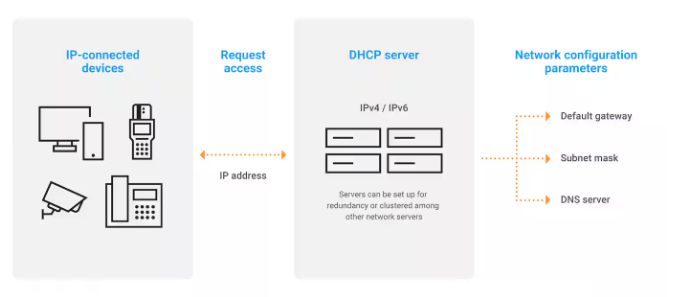
\includegraphics[width=0.7\linewidth]{image/1.png}
            \caption{Giao thức DHCP (Dynamic Host Configuration Protocol)}
            \label{fig:label1}
    \end{figure}
    \begin{itemize}
        \item Dynamic Host Configuration Protocol (DHCP - giao thức cấu hình động máy chủ) là một giao thức cung cấp phương pháp thiết lập động các thông số cần thiết cho hoạt động của mạng TCP/IP, giúp giảm khối lượng công việc cho người quản trị hệ thống. Cơ chế cấp phát động các thông số mạng có ưu điểm hơn cơ chế khai báo tĩnh là:
        \begin{itemize}
            \item Khắc phục được tình trạng trùng địa chỉ IP.
            \item Giảm chi phí cho quản trị hệ thống mạng.
            \item Tiết kiệm và tận dụng tốt nhất số lượng địa chỉ IP public mà nhà cung cấp đã phân phát.
            \item Có thể kết hợp được với sử dụng mạng Wireless.
        \end{itemize}
        \item Trong một hệ thống mạng các máy tính liên lạc với nhau bằng Protocol TCP/IP do đó các máy tính này phải được cấu hình theo một thông số IP nhất định.
    \end{itemize}

    \item \textbf{Hệ thống phân giải tên miền DNS (Domain Name System)}
    \begin{figure}[h!]
        \centering
        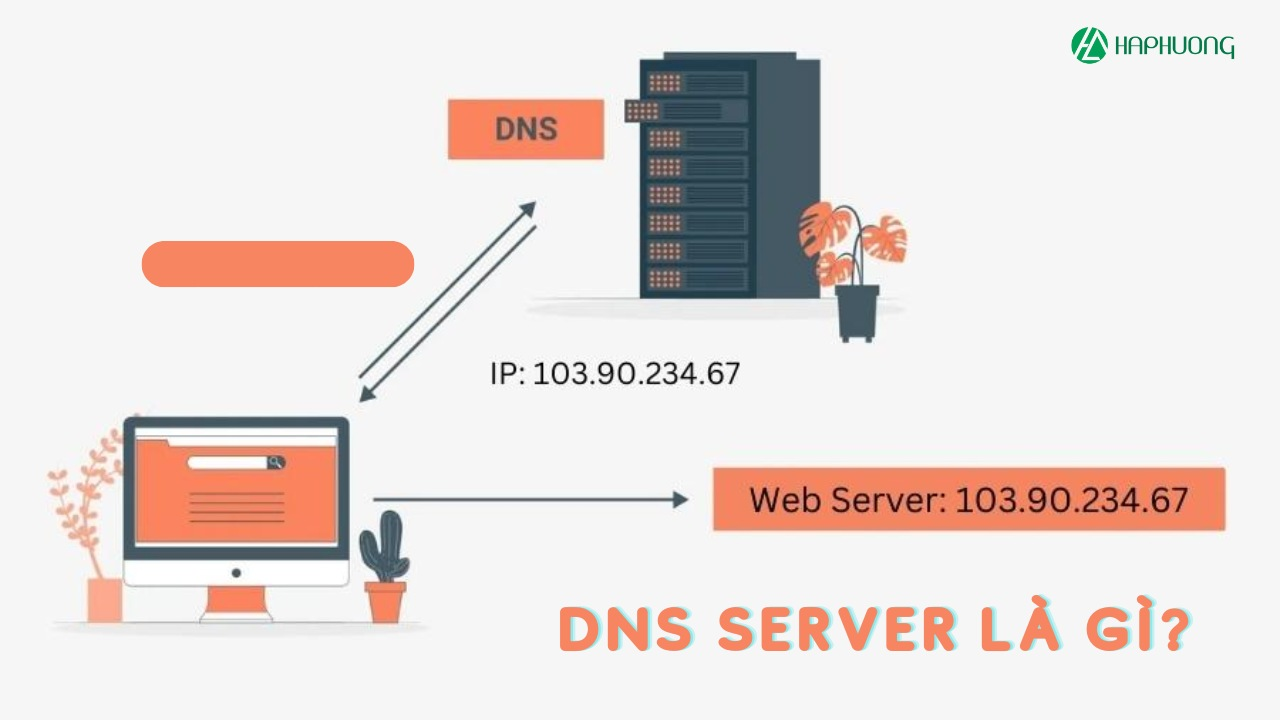
\includegraphics[width=0.7\linewidth]{image/2.jpg}
            \caption{Hệ thống phân giải tên miền DNS (Domain Name System)}
            \label{fig:label1}
    \end{figure}
    
    \begin{itemize}
        \item Mỗi Website có một tên (là tên miền hay đường dẫn URL Uniform Resource Locator) và một địa chỉ IP. Địa chỉ IP gồm 4 nhóm số cách nhau bằng dấu chấm(IPv4). Khi mở một trình duyệt Web và nhập tên website, trình duyệt sẽ đến thẳng website mà không cần phải thông qua việc nhập địa chỉ IP của trang web. 
        \item Quá trình "dịch" tên miền thành địa chỉ IP để cho trình duyệt hiểu và truy cập được vào website là công việc của một DNS server. Các DNS trợ giúp qua lại với nhau để dịch địa chỉ "IP" thành "tên" và ngược lại. Người sử dụng chỉ cần nhớ "tên", không cần phải nhớ địa chỉ IP.
    \end{itemize}

    \item \textbf{Dịch vụ FTP (File Transfer Protocol)}
    \begin{figure}[h!]
        \centering
        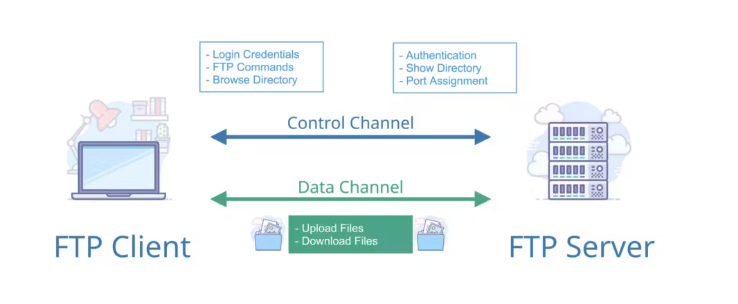
\includegraphics[width=0.7\linewidth]{image/3.png}
            \caption{Dịch vụ FTP (File Transfer Protocol)}
            \label{fig:label1}
    \end{figure}
    
    \begin{itemize}
        \item FTP (File Transfer Protocol) là một dịch vụ cho phép ta truyền tải file giữa hai máy tính ở xa dùng giao thức TCP/IP. FTP cũng là một ứng dụng theo mô hình client-server, nghĩa là máy làm FTP Server sẽ quản lý các kết nối và cung cấp dịch vụ tập tin cho các máy trạm.
        \item Nói tóm lại FTP Server thường là một máy tính phục vụ cho việc quảng bá các tập tin cho người dùng hoặc là một nơi cho phép người dùng chia sẻ tập tin với những người dùng khác trên Internet. Máy trạm muốn kết nối vào FTP Server thì phải được Server cấp cho một account có đầy đủ các thông tin như: địa chỉ máy Server (tên hoặc địa chỉ IP), username và password. 
        \item Phần lớn các FTP Server cho phép các máy trạm kết nối vào mình thông qua account anonymous (account anonymous thường được truy cập với password rỗng). Các máy trạm có thể sử dụng các lệnh ftp đã tích hợp sẵn trong hệ điều hành hoặc phần mềm chuyên dụng khác để tương tác với máy FTP Server.
    \end{itemize}
    
    \item \textbf{Dịch vụ Web}
    \begin{figure}[h!]
        \centering
        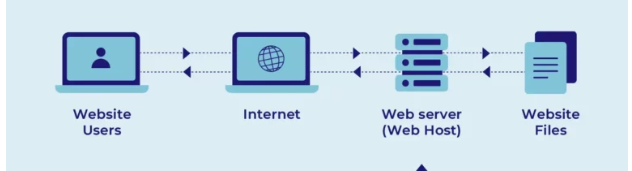
\includegraphics[width=0.7\linewidth]{image/4.png}
            \caption{Dịch vụ Web}
            \label{fig:label1}
    \end{figure}
    
    \begin{itemize}
        \item Là một mô-đun phần mềm được thiết kế để thực hiện một nhóm các tác vụ nhất định. Các web services có thể được truy cập và sử dụng thông qua mạng internet dưới dạng dịch vụ. Khi đó, web service sẽ cung cấp các chức năng của nó cho máy khách để người dùng đạt được các mục tiêu sử dụng nhất định. Ta có thể hiểu, để một dịch vụ được coi là web service thì cần thỏa mãn các tiêu chí sau:
        \begin{itemize}
            \item Có sẵn ở trên internet hoặc trong mạng nội bộ.
            \item Sử dụng một hệ thống XML messaging đúng tiêu chuẩn
            \item Hoàn toàn không bị trói buộc bởi một hệ điều hành hay ngôn ngữ lập trình nào
            \item Có thể tự diễn tả thông qua một cấu trúc XML đơn giản
            \item Được tìm kiếm dễ dàng bằng những phương thức đơn giản (simple mechanism).
        \end{itemize}	
    \end{itemize}

    \item \textbf{Dịch vụ Mail Server}
    \begin{figure}[h!]
        \centering
        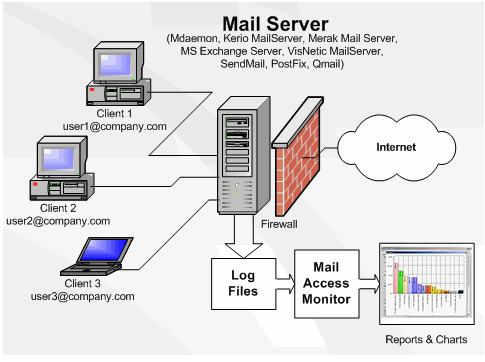
\includegraphics[width=0.7\linewidth]{image/5.png}
            \caption{Dịch vụ Mail Server}
            \label{fig:label1}
    \end{figure}
    
    \begin{itemize}
        \item Mail Server hay Email Server là hệ thống máy chủ được cấu hình riêng theo tên miền của doanh nghiệp dùng để gửi và nhận thư điện tử. 
        \item Bên cạnh tính năng lưu trữ và sắp xếp các Email trên internet, Mail Server là một giao thức chuyên nghiệp để giao tiếp thư tín, quản lý và truyền thông nội bộ, giao dịch thương mại, ... 
        \item Không chỉ thao tác với tốc độ nhanh chóng và ổn định, Mail Server còn đảm bảo tính an toàn với khả năng khôi phục dữ liệu cao.
    \end{itemize}
    
\end{enumerate}

\subsubsection{Các kiểu topology của mạng LAN}
\begin{enumerate}
    \item \textbf{Loại hình tuyến - Bus Topology (logic)}
    \begin{figure}[h!]
        \centering
        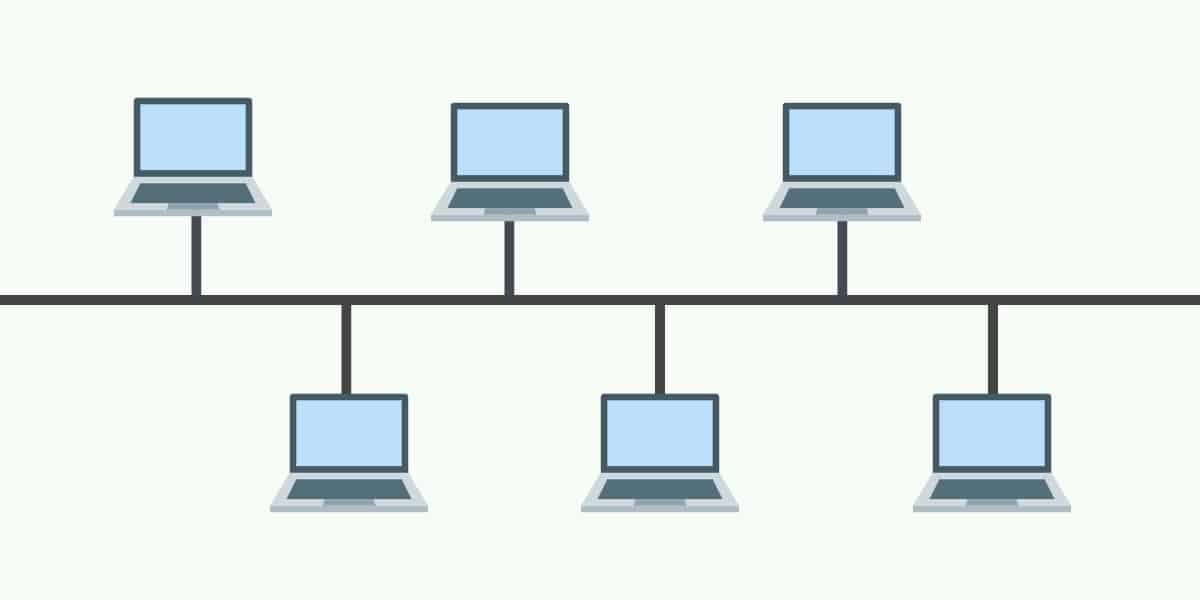
\includegraphics[width=0.7\linewidth]{image/6.jpg}
            \caption{Loại hình tuyến - Bus Topology (logic)}
            \label{fig:label1}
    \end{figure}

    \begin{itemize}
        \item Bus Topology cũng là một trong các kiểu kết nối mạng được sử dụng rất phổ biến. Mô hình này giúp cho máy chủ và hệ thống máy tính hoặc các nút thông tin được kết nối cùng nhau trên một trục đường dây cáp chính. Mục đích của sự kết nối này là nhằm chuyển tải các tín hiệu thông tin.
        \item Thông thường ở phía hai đầu của dây cáp sẽ được bịt kín bằng thiết bị terminator. Riêng các tín hiệu và gói dữ liệu di chuyển trong dây cáp sẽ mang theo địa chỉ của điểm đến.
        \item Ưu điểm nổi bật nhất của mạnh hình tuyến chính là việc tiết kiệm chiều dài dây cáp và rất dễ lắp đặt. Nhưng mô hình mạng cũng tồn tại những khuyết điểm điển hình như dễ gây ra sự ùn tắc giao thông trong quá trình di chuyển dữ liệu số lượng lớn. Một khi có sự cố hư hỏng xảy ra ở đoạn cáp nào đó, user sẽ rất khó phát hiện. Vì vậy bạn bắt buộc phải tạm ngừng hoạt động trên đường dây và toàn bộ hệ thống để tiến hành sửa chữa.
    \end{itemize}

    \item \textbf{Loại hình vòng - Ring Topology (logic)}
    \begin{figure}[h!]
        \centering
        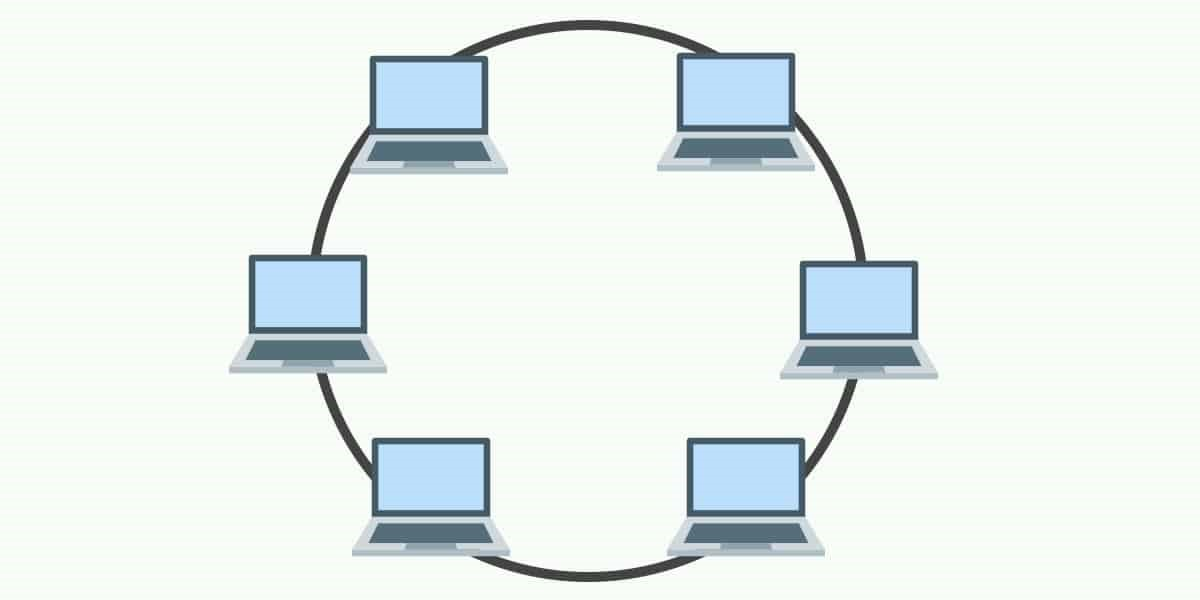
\includegraphics[width=0.7\linewidth]{image/11.jpg}
            \caption{Loại hình vòng - Ring Topology (logic)}
            \label{fig:label1}
    \end{figure}

    \begin{itemize}
        \item Mô hình mạng LAN dạng vòng được bố trí theo dạng xoay vòng. Trong trường hợp này, đường dây cáp sẽ được thiết kế thành vòng tròn khép kín. Các tín hiệu chạy quanh vòng tròn sẽ di chuyển theo một chiều nào đó cố định.
        \item Bên trong mạng dạng vòng, tại mỗi một thời điểm nhất định chỉ có một nút có khả năng truyền tín hiệu trong số hệ thống các nút thông tin. Song song đó, dữ liệu truyền đi cũng phải kèm theo địa chỉ đến tại mỗi trạm tiếp nhận.
        \item Ưu điểm của mạng dạng vòng chính là có thể nới rộng hệ thống mạng ra xa. Số lượng dây dẫn cần thiết để sử dụng cũng ít hơn so với hai mô hình mạng kể trên. Tuy nhiên khuyết điểm lớn nhất của kiểu mạng dạng vòng chính là đường dây phi khép kín. Một khi tín hiệu bị ngắt tại một điểm nào đó, toàn bộ hệ thống cũng sẽ ngừng hoạt động.
    \end{itemize}

    \item \textbf{Loại hình sao - Star Topology (physical)}

    \begin{itemize}
        \item Star Topology là mạnh dạng hình sao có một trung tâm và các nút thông tin. Bên trong mạng, các nút thông tin là những trạm đầu cuối. Đôi khi nút thông tin cũng chính là hệ thống các máy tính và những thiết bị khác của mạng LAN.
     \begin{figure}[h!]
        \centering
        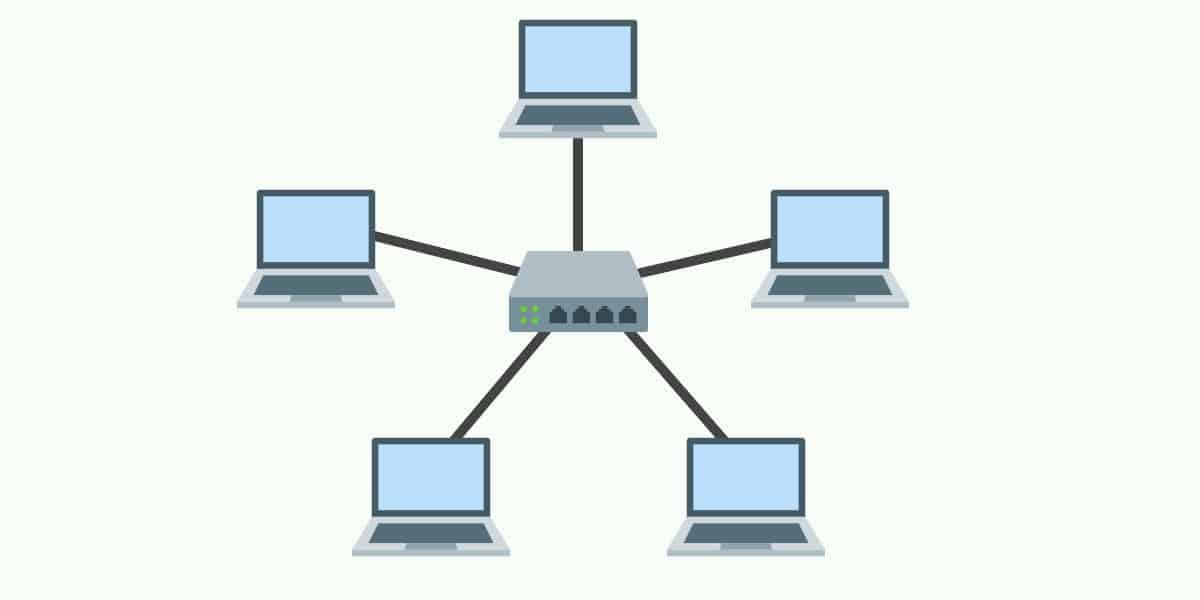
\includegraphics[width=0.7\linewidth]{image/7.jpg}
            \caption{Loại hình sao - Star Topology (physical)}
            \label{fig:label1}
    \end{figure}
    
        \item Khu vực trung tâm mạng dạng hình sao đảm nhận nhiệm vụ điều phối mọi hoạt động bên trong hệ thống. Bộ phận này mang các chức năng cơ bản là:
        \begin{itemize}
            \item Nhận dạng những cặp địa chỉ gửi và nhận có quyền chiếm tuyến thông tin và tiến hành quá trình liên lạc với nhau.
            \item Phê duyệt quá trình theo dõi và xử lý khi các thiết bị trao đổi thông tin với nhau.
            \item Gửi đi các thông báo về trạng thái của mạng LAN.
        \end{itemize}
    
    \item Ưu điểm của mạng hình sao:
        \begin{itemize}
            \item Mô hình mạng LAN dạng hình sao đảm bảo quá trình hoạt động bình thường khi có một nút thông tin bị hư hỏng. Bởi kiểu mạng LAN này hoạt động dựa trên nguyên lý song song.
            \item Đặc điểm cấu trúc mạng vô cùng đơn giản. Điều này giúp cho thuật toán được điều khiển một cách ổn định hơn.
            \item Tùy vào nhu cầu sử dụng của User, mạnh dạng hình sao có thể được mở rộng hoặc thu hẹp theo ý muốn.
        \end{itemize}
    \item Nhược điểm của mạng hình sao:
        \begin{itemize}
            \item Mặc dù có khả năng mở rộng mạng, nhưng điều này hoàn toàn phụ thuộc vào khả năng hoạt động của bộ phận trung tâm. Một khi trung tâm gặp phải sự cố, toàn bộ hệ thống mạng sẽ không thể hoạt động.
            \item Mạnh dạng hình sao yêu cầu phải được kết nối một cách độc lập với từng thiết bị ở nút thông tin đến trung tâm. Song song đó là khoảng cách kết nối từ thiết bị đến trung tâm cũng rất hạn chế và thường chỉ đạt khoảng 100m.
            \item Nhìn một cách tổng quan, mô hình mạng dạng hình sao giúp cho các máy tính kết nối với bộ tập trung (HUB) bằng cáp xoắn. Kiểu kết nối trên cho phép việc kết nối máy tính trực tiếp với HUB mà không cần thông qua trục BUS. Nhờ vậy mà hệ thống mạng hạn chế tối đa các yếu tố gây ngưng trệ mạng trong quá trình hoạt động.
        \end{itemize}
    \end{itemize}

    \item \textbf{Loại hình lưới - Mesh Topology (physical và logic)}
    \begin{figure}[h!]
        \centering
        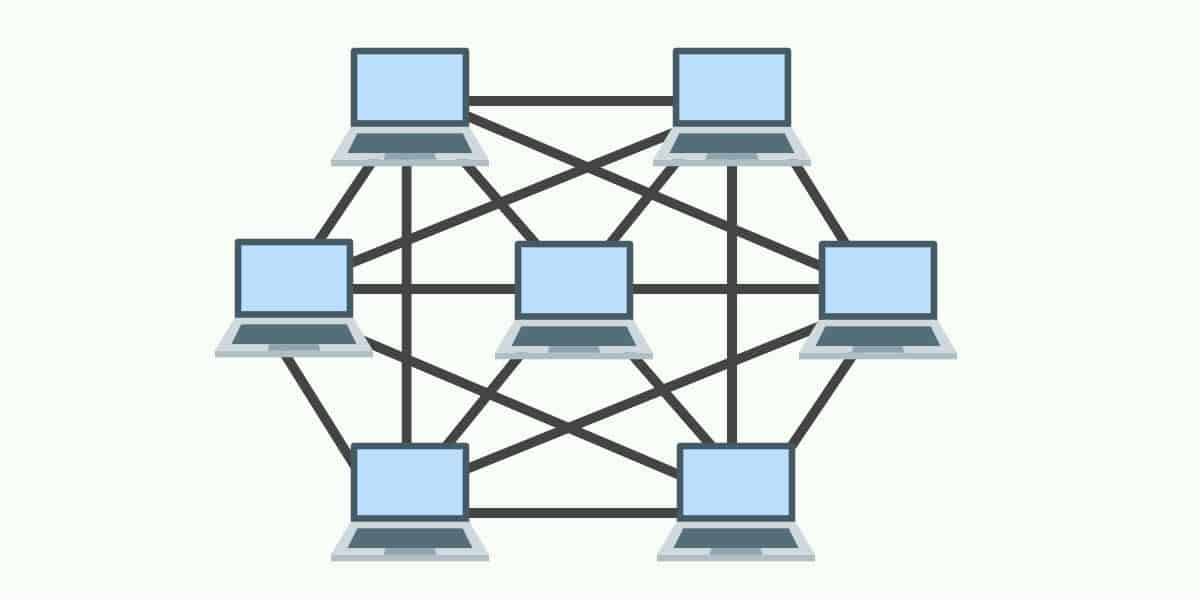
\includegraphics[width=0.7\linewidth]{image/8.jpg}
            \caption{Loại hình lưới - Mesh Topology (physical và logic)}
            \label{fig:label1}
    \end{figure}

    \begin{itemize}
        \item Mesh Topology hay còn gọi là mạnh dạng lưới. Sản phẩm có cấu trúc dạng lưới được ứng dụng phổ biến trong các mạng nắm giữ vai trò quan trọng và không thể bị ngừng hoạt động. Điển hình như hệ thống mạng của nhà máy điện nguyên tử hoặc hệ thống mạng an ninh, quốc phòng.
        \item Đối với mạng dạng lưới, mỗi một thiết bị máy tính sẽ được kết nối với tất cả cả các máy tính còn lại. Đó cũng là cấu trúc quen thuộc của mạng Internet.
    \end{itemize}

    \item \textbf{Loại hình sao mở rộng}
    \begin{figure}[h!]
        \centering
        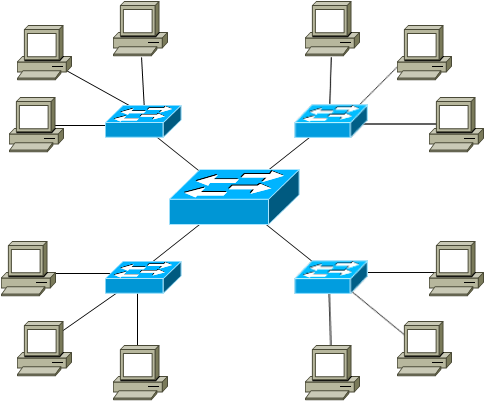
\includegraphics[width=0.7\linewidth]{image/9.png}
            \caption{Loại hình sao mở rộng}
            \label{fig:label1}
    \end{figure}
    
    \begin{itemize}
        \item Khác với các mô hình mạng kể trên, mạng hình sao mở rộng là sự kết hợp giữa các mạng hình sao với nhau, thông qua việc kết nối các HUB hoặc Switch. Ưu điểm của mạng hình sao mở rộng chính là có thể gia tăng khoảng cách hay độ lớn của mạng hình sao.
    \end{itemize}

    \newpage
    \item \textbf{Loại hình cấu trúc cây - Hierachical Topology}
    \begin{figure}[h!]
        \centering
        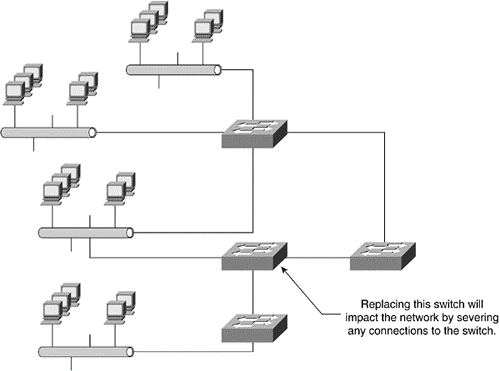
\includegraphics[width=0.7\linewidth]{image/10.png}
            \caption{Loại hình cấu trúc cây - Hierachical Topology}
            \label{fig:label1}
    \end{figure}
    
    \begin{itemize}
        \item Mạng có cấu trúc cây sở hữu đặc điểm cấu tạo như mạng hình sao mở rộng. Nhưng thay vì liên kết các Switch hoặc HUB với nhau, thì hệ thống mạng lại kết nối với một thiết bị máy tính mang nhiệm vụ kiểm tra sự lưu của hệ thống mạng.
    \end{itemize}
\end{enumerate}
\subsection{Công nghệ VLAN (Virtual Local Area Network)}
    \begin{figure}[h!]
        \centering
        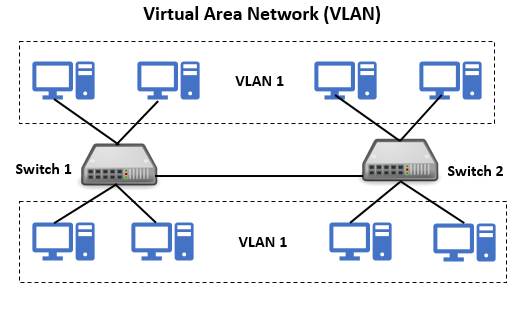
\includegraphics[width=0.7\linewidth]{image/12.png}
            \caption{VLAN (Virtual Local Area Network)}
            \label{fig:label1}
    \end{figure}
    
\subsubsection{Khái niệm}
\begin{itemize}
    \item Trước khi tìm hiểu về VLAN ta phải hiểu LAN là gì? LAN là một mạng cục bộ (viết tắt của Local Area Network), được định nghĩa là tất cả các máy tính trong cùng một miền quảng bá (broadcast domain).
    \item Các router (bộ định tuyến) chặn bản tin quảng bá, trong khi switch (bộ chuyển mạch) chỉ chuyển tiếp chúng.
    \item VLAN là một mạng LAN ảo. Về mặt kỹ thuật, VLAN là một miền quảng bá được tạo bởi các switch. Bình thường thì router đóng vai trò tạo ra miền quảng bá. Đối với VLAN, switch có thể tạo ra miền quảng bá.
    \item Bạn có thể hiểu dễ hơn là VLAN dùng để chia một con Switch thành nhiều con Switch nhỏ hơn và hoàn toàn độc lập với nhau.
    \begin{itemize}
        \item Với network: VLAN = Broadcast domain = Logical Network 
        \item Với Switch: VLAN = Logical switch.
    \end{itemize}
    \item Một Switch có thể tạo ra nhiều VLAN, khi switch có một broadcast được gửi bởi một thiết bị nằm trong một VLAN sẽ được chuyển đến những thiết bị khác trong cùng VLAN, tuy nhiên broadcast sẽ không được forward đến các thiết bị trong VLAN khác.
\end{itemize}

\subsubsection{Phân loại}
\begin{itemize}
    \item Mạng VLAN gồm có 3 loại chính như sau:
    \begin{itemize}
        \item \textbf{Port - based VLAN:} là cách cấu hình VLAN đơn giản và phổ biến. Mỗi cổng của Switch được gắn với một VLAN xác định (mặc định là VLAN 1), do vậy bất cứ thiết bị host nào gắn vào cổng đó đều thuộc một VLAN nào đó.
        \item \textbf{MAC address based VLAN:} Cách cấu hình này ít được sử dụng do có nhiều bất tiện trong việc quản lý. Mỗi địa chỉ MAC được đánh dấu với một VLAN xác định.
        \item \textbf{Protocol – based VLAN:} Cách cấu hình này gần giống như MAC Address based, nhưng sử dụng một địa chỉ logic hay địa chỉ IP thay thế cho địa chỉ MAC. Cách cấu hình không còn thông dụng nhờ sử dụng giao thức DHCP
    \end{itemize}
\end{itemize}

\subsubsection{Ưu, nhược điểm của VLAN}
\begin{enumerate}
    \item \textbf{Ưu điểm:}
\begin{itemize}
    \item Tiết kiệm băng thông của mạng: Do VLAN có thể chia nhỏ LAN thành các đoạn khác nhau.
    \item Khi gửi 1 gói tin , nó sẽ chỉ gửi trong một VLAN duy nhất, không truyền ở các VLAN khác nên giảm được lưu lượng, tiết kiệm được băng thông đường truyền, không làm giảm tốc độ đường truyền.
    \item Tăng khả năng bảo mật: Các VLAN khác nhau không truy cập được vào nhau (trừ khi có khai báo định tuyến). Nếu có sự cố của một VLAN cuãng không làm ảnh hưởng tới VLAN khác.
    \item Dễ dàng thêm hay bớt các máy tính vào VLAN: Trên một switch nhiều cổng, có thể cấu hình VLAN khác nhau cho từng cổng, do đó dễ dàng kết nối thêm các máy tính với các VLAN.
    \item Mạng có tính linh động cao: VLAN có thể dễ dàng di chuyển các thiết bị. VLAN có thể được cấu hình tĩnh hay động. Trong cấu hình tĩnh, người quản trị mạng phải cấu hình cho từng cổng của mỗi switch. Sau đó, gán cho nó vào một VLAN nào đó. Trong cấu hình động mỗi cổng của switch có thể tự cấu hình VLAN cho mình dựa vào địa chỉ MAC của thiết bị được kết nối vào.
    \item Mạng VLAN đem lại rất nhiều lợi ích giúp giảm tải và chia đều người truy cập internet nhất là đối với những máy tính có dung lượng lớn, nhiều người truy cập vào một lúc để người dùng có thể truy cập internet nhanh hơn. Mạng VLAN thường được áp dụng với các công ty lớn khi lượng truy cập internet cùng lúc quá nhiều.
\end{itemize}

\item \textbf{Nhược điểm:}
\begin{itemize}
    \item Gói tin có thể bị rò rỉ giữa các VLAN.
    \item Để xử lý được khối công việc trong hệ thống mạng lớn, cần có thiết bị định tuyến mạnh.
    \item Một VLAN không thể chuyển tiếp lưu lượng mạng tới những VLAN khác.
    \item Khả năng tương tác là một rào cản lớn.
    \item Các mối đe dọa trong hệ thống đơn lẻ có thể phát tán virus khắp hệ thống mạng.
    \item Cấu hình VLAN phải phụ thuộc nhiều vào nhà sản xuất thiết bị mạng do tiêu chuẩn chính thức  IEEE 802.1q chưa được phê duyệt.
\end{itemize}
\end{enumerate}


\subsubsection{Khi nào cần VLAN?}
\begin{itemize}
    \item Cần cân nhắc việc sử dụng VLAN trong các trường hợp sau:
    \begin{itemize}
        \item Khi có hơn 200 máy tính trong mạng LAN.
        \item Lưu lượng quảng bá (broadcast traffic) trong mạng LAN quá lớn.
        \item Các nhóm làm việc cần gia tăng bảo mật hoặc bị làm chậm vì quá nhiều bản tin quảng bá.
        \item Các nhóm làm việc cần nằm trên cùng một miền quảng bá vì họ đang dùng chung các ứng dụng. Ví dụ như một công ty sử dụng điện thoại VoIP. Một số người muốn sử dụng điện thoại có thể thuộc một mạng VLAN khác, không cùng với người dùng thường xuyên.
        \item Chuyển đổi một switch đơn thành nhiều switch ảo.
    \end{itemize}
\end{itemize}

\subsection{Công nghệ VXLAN (Virtual Extensible LAN)}
\subsubsection{Đặt vấn đề}
Trước đây, các trung tâm dữ liệu sử dụng VLAN để cô lập mạng lớp 2 (L2). Tuy nhiên, với sự mở rộng không ngừng của các trung tâm dữ liệu, việc mở rộng mạng lớp 2 ra trung tâm dữ liệu ngày càng trở nên quan trọng. Những hạn chế của VLAN đã trở nên rõ ràng và phải nhanh chóng được khắc phục. Cụ thể, các hạn chế của VLAN bao gồm:
\begin{itemize}
    \item \textbf{Hạn chế về số lượng VLAN trong trung tâm dữ liệu:} Trong các trung tâm dữ liệu, có thể yêu cầu hàng ngàn VLAN để phân tách lưu lượng trong các môi trường ảo dùng chung các siêu thị mạng lớp 2 và lớp 3(L2/L3). Lớp 2 (L2) là tầng liên kết dữ liệu, nơi quản lý việc chuyển gói tin trong cùng một mạng cục bộ,còn lớp 3 (L3) là tầng mạng, xử lý việc định tuyến các gói tin giữa các mạng khác nhau. Giới hạn 4096 VLAN, trong đó một số VLAN dùng để dự trữ, không đủ để đáp ứng nhu cầu này.
    \item \textbf{Vấn đề về bảng địa chỉ MAC trong máy chủ ảo:} Mỗi máy chủ ảo yêu cầu một địa chỉ MAC và một địa chỉ IP riêng biệt. Điều này dẫn đến việc có hàng ngàn mục trong bảng địa chỉ MAC trên các thiết bị chuyển mạch upstream, tạo ra nhu cầu lớn hơn về dung lượng của bảng địa chỉ và bộ nhớ quản lý mạng.
    \item \textbf{Hạn chế về khả năng cải và triển khai VLAN:} VLAN bị hạn chế về khả năng cách trình thiết lập linh hoạt. Mặc dù giao thức VTP có thể được sử dụng để triển khai VLAN qua các switch lớp 2, nhưng lại hết sức hạn chế khi không có chúng VTP do những hạn chế về rủi ro do cấu hình tự động có thể gây ra các vấn đề về khả năng mở rộng của cấu hình mạng nếu không được quản lý cẩn thận.
    \item \textbf{Vấn đề về khả năng chịu lỗi và hiệu suất của VLAN:} VLAN bị giới hạn về khả năng cung cấp một topology lớp 2 chống loop bằng cách diễn lại việc nối lại các liên kết và kiểm soát broadcast. Với các mạng lớp 3, việc triển khai ECMP để cải thiện khả năng chịu lỗi là một khó khăn. Trong khi đó, ECMP có thể được sử dụng rộng rãi trong mạng lớp 3, cho phép tối ưu hóa lưu lượng và tăng cường hiệu suất bằng cách dùng thông.
\end{itemize}

\subsubsection{VXLAN - Giải pháp cho các hạn chế của VLAN}
\begin{itemize}
    \item VXLAN là một công nghệ mạng được phát triển để giải quyết những hạn chế của VLAN truyền thống. VLAN cho phép phân chia mạng vật lý thành nhiều mạng ảo hơn, tuy nhiên, hạn chế của VLAN bao gồm giới hạn về số lượng VLAN có thể triển khai (tối đa 4094 VLAN) và khả năng mở rộng chưa linh hoạt trên các mạng vật lý phức tạp.

    \begin{figure}[h!]
        \centering
        \includegraphics[width=0.7\linewidth]{image/VTEP_structure.png}
            \caption{Mô hình hoạt động VXLAN}
            \label{fig:label1}
    \end{figure}
    
    \item Với sự bùng nổ của các ứng dụng đám mây và các mô hình mạng phân tán, nhu cầu mở rộng mạng lớp 2 qua mạng lớp 3 trở nên cấp thiết hơn bao giờ hết. Đây là nơi mà VXLAN ra đời như một giải pháp hiệu quả. (Mahalingam et al., 2014) VXLAN cho phép tạo ra các mạng ảo một cách độc lập trên hạ tầng mạng hiện có, mở rộng mạng lớp 2 một cách linh hoạt trên các mạng lớp 3 khác nhau, bằng cách sử dụng giao thức UDP để truyền dữ liệu và chèn thêm địa chỉ IP vào gói tin lớp 2. Điều này tạo ra các đường hầm (tunnel) VXLAN giúp kết nối các mạng ảo với nhau và với mạng vật lý một cách hiệu quả.
    \item VXLAN cung cấp dịch vụ kết nối Ethernet tới các thiết bị đầu cuối tương tự như VLAN, nhưng với nhiều tính năng mở rộng hơn. Trong khi chuẩn VLAN 802.1q chỉ sử dụng 12 bit để đánh số VLAN-ID, VXLAN sử dụng tới 24 bit, tạo ra không gian địa chỉ lớn hơn nhiều lần, cho phép hỗ trợ hơn 16 triệu địa chỉ. Điều này đảm bảo đủ không gian để triển khai các mạng có quy mô lớn trong tương lai.
    \item VXLAN sử dụng giao thức IP (bao gồm cả unicast và multicast) để truyền dẫn. Sự phổ biến của mạng IP và các thiết bị đầu cuối hỗ trợ IP cho phép VXLAN có khả năng mở rộng vượt trội, xa hơn nhiều so với VLAN sử dụng chuẩn 802.1q hiện nay. VXLAN đã được phát triển để khắc phục các vấn đề của VLAN và đáp ứng nhu cầu mở rộng mạng của các trung tâm dữ liệu hiện đại. VXLAN cung cấp các lợi ích chính sau:
    \begin{itemize}
        \item Mở rộng không gian địa chỉ VLAN: VXLAN mở rộng không gian địa chỉ VLAN từ 4096 lên tới 16 triệu, cho phép tạo ra nhiều mạng ảo và phân tách lưu lượng hiệu quả hơn trong các trung tâm dữ liệu lớn.
        \item Hỗ trợ tốt hơn cho ảo hóa: VXLAN hỗ trợ tốt hơn cho các môi trường ảo hóa, cho phép các máy ảo di chuyển tự do giữa các máy chủ và trung tâm dữ liệu mà không gặp trở ngại về các trục trặc mạng.
        \item Khả năng mở rộng và triển khai linh hoạt: VXLAN sử dụng giao thức UDP để encapsulate các khung Ethernet trong các gói IP, cho phép triển khai linh hoạt qua mạng lớp 3 và mở rộng cách triển khai mà không bị giới hạn bởi các ràng buộc vật lý của VLAN.
        \item Hỗ trợ ECMP: VXLAN hỗ trợ ECMP, cho phép tối ưu hóa lưu lượng và sử dụng băng thông hiệu quả
hơn trong các mạng trung tâm dữ liệu.
    \end{itemize}
\end{itemize}

\subsubsection{Các khái niệm trong VXLAN}
\begin{enumerate}
    \item \textbf{Virtual Network Identifier (VNI)}
    \begin{itemize}
        \item Virtual Network Identifier là một giá trị được sử dụng để xác định một mạng ảo cụ thể trong một phạm vi dữ liệu của VXLAN. VNI là một phần của tiêu đề VXLAN và có kích thước 24 bit, cho phép hỗ trợ lên đến 16 triệu phân đoạn mạng riêng lẻ (từ giá trị 4096 đến 16.777.215).
        \item VNI xác định phạm vi của inner MAC frame sinh ra bởi máy ảo VM. Điều này có nghĩa là địa chỉ MAC có thể được overlap giữa các phân đoạn mạng khác nhau mà không gây xung đột, vì các lưu lượng này là cô lập bởi các VNI khác nhau. Cho phép cách ly một số lượng lớn người dùng mạng trên cùng một cơ sở hạ tầng vật lý. Người dùng trên các phân đoạn VXLAN khác nhau không thể giao tiếp ở lớp 2, trừ khi được cấu hình để kết nối thông qua một router.
        \item  VNI tương tự như VLAN ID trong mạng truyền thống. Tuy nhiên, trong khi VLAN ID có giới hạn về số lượng (4096), VNI mở rộng khả năng này lên đến 16 triệu phân đoạn. Điều này làm cho VXLAN trở nên đặc biệt hữu ích trong các mạng lớn. Khi một gói tin được truyền qua VXLAN, VNI 24-bit được thêm vào tiêu đề của gói VXLAN. Điều này cho phép VXLAN cách ly và quản lý lưu lượng của nhiều người dùng khác nhau một cách hiệu quả. VXLAN hoạt động như một lớp overlay, tạo ra một mạng lớp 2 trên hạ tầng mạng lớp 3 hiện có. Mỗi phân đoạn mạng VXLAN được xác định bởi VNI, chỉ các máy ảo trong cùng một phân đoạn mới có thể giao tiếp với nhau.
    \end{itemize}
    
    \item \textbf{Định dạng gói và đóng gói VXLAN (Encapsulation and Packet Format)}
    \begin{itemize}
        \item VXLAN là một giải pháp hỗ trợ môi trường đa thuê bao linh hoạt và quy mô lớn trên một cơ sở hạ tầng vật lý chung. Trong mạng trung tâm dữ liệu vật lý, giao thức vận chuyển được sử dụng là IP cộng với UDP. VXLAN định nghĩa một sơ đồ đóng gói gọi là MAC-in-UDP, trong đó khung lớp 2 gốc được thêm một tiêu đề VXLAN và sau đó được đặt trong một gói UDP-IP. Điều này cho phép VXLAN tạo các đường hầm mạng lớp 2 qua mạng lớp 3, mang lại sự linh hoạt và mở rộng cho mạng ảo hóa.
        \item Tiêu đề VXLAN dài 8 byte và bao gồm một VNID 24 bit cùng với một số bit dự trữ. Tiêu đề VXLAN cùng với khung Ethernet gốc được đặt trong tải trọng UDP. VNID 24 bit được sử dụng để xác định các phân đoạn lớp 2 và duy trì sự cách ly giữa các phân đoạn này. Với 24 bit trong VNID, VXLAN có thể hỗ trợ lên đến 16 triệu phân đoạn LAN, giúp mở rộng khả năng mạng một cách đáng kể.
        \item VXLAN hoạt động bằng cách đóng gói khung lớp 2 gốc với một tiêu đề VXLAN, sau đó đặt toàn bộ khung này vào trong một gói UDP-IP. Quá trình này cho phép mạng lớp 2 được truyền tải qua mạng lớp 3, giữ nguyên tính toàn vẹn và cách ly của các phân đoạn lớp 2. Điều này đặc biệt quan trọng trong các môi trường đa thuê bao, nơi sự cách ly và bảo mật giữa các thuê bao là rất cần thiết. Với định dạng gói và đóng gói này, VXLAN cung cấp một phương thức hiệu quả và linh hoạt để mở rộng và quản lý các mạng ảo trên cơ sở hạ tầng vật lý hiện có.
    \end{itemize}

    \item \textbf{VXLAN Tunnel Endpoint}
    \begin{figure}[h!]
        \centering
        \includegraphics[width=0.7\linewidth]{image/VTEP_structure.png}
            \caption{VXLAN Tunnel Endpoint)}
            \label{fig:label1}
    \end{figure}
    
    \begin{itemize}
        \item VXLAN sử dụng các điểm cuối đường hầm VXLAN, hay còn gọi là VTEP, để ánh xạ các thiết bị đầu cuối của người thuê vào các phân đoạn VXLAN, đồng thời thực hiện việc đóng gói và giải đóng gói VXLAN. Mỗi VTEP có hai giao diện quan trọng: một giao diện chuyển mạch trên phân đoạn LAN cục bộ để hỗ trợ giao tiếp giữa các điểm cuối cục bộ và một giao diện IP kết nối tới mạng truyền tải IP.
        \item Trong mạng truyền tải IP, mỗi VTEP được xác định bằng một địa chỉ IP duy nhất gọi là VLAN hạ tầng. Thiết bị VTEP sử dụng địa chỉ IP này để đóng gói các khung Ethernet và truyền các gói tin đã được đóng gói đến mạng truyền tải thông qua giao diện IP. Điều này đảm bảo rằng các gói tin có thể di chuyển một cách hiệu quả và chính xác giữa các phân đoạn mạng khác nhau.
        \item Bên cạnh đó, thiết bị VTEP cũng có khả năng phát hiện các VTEP từ xa cho các phân đoạn VXLAN của mình và học các ánh xạ địa chỉ MAC từ xa tới VTEP thông qua giao diện IP. Quá trình này giúp duy trì sự liên kết và kết nối giữa các phân đoạn mạng khác nhau, đảm bảo tính toàn vẹn và hiệu quả của mạng VXLAN. Các thành phần chức năng của VTEP và cấu trúc liên kết logic được thiết lập để cung cấp kết nối lớp 2 qua mạng truyền tải IP được mô tả rõ ràng trong các sơ đồ cấu trúc, chẳng hạn như trong hình bên dưới.
    \end{itemize}
\end{enumerate}

\subsubsection{Cổng VXLAN}
\begin{itemize}
    \item Cổng VXLAN được sử dụng để kết nối các phân đoạn VXLAN và VLAN truyền thống, tạo ra một miền chuyển tiếp thống nhất, cho phép các thiết bị thuê bao hoạt động trong cả hai môi trường. Các loại cổng VXLAN bao gồm:
    \begin{itemize}
        \item Cổng VXLAN Lớp 2: Đây là thiết bị chịu trách nhiệm đóng gói các khung Ethernet truyền thống (Classical Ethernet - CE) thành khung VXLAN và ngược lại. Thiết bị cổng này cung cấp các lợi ích của VXLAN cho các thiết bị không hỗ trợ VXLAN một cách minh bạch, bao gồm cả các máy chủ vật lý và máy ảo. Các thiết bị này hoàn toàn không nhận biết được việc đóng gói VXLAN.
        \item Cổng VXLAN Lớp 3: Giống như việc định tuyến giữa các VLAN khác nhau, cần có một bộ định tuyến VXLAN để kết nối các thiết bị trong các phân đoạn VXLAN khác nhau. Bộ định tuyến này chuyển đổi các khung từ VNI này sang VNI khác, và quá trình này có thể bao gồm giải đóng gói và đóng gói lại khung tùy thuộc vào nguồn và đích. Thiết bị Cisco Nexus hỗ trợ tất cả các tổ hợp của quá trình giải đóng gói, định tuyến và đóng gói lại. Việc định tuyến cũng có thể được thực hiện trên các giao diện lớp 3 gốc và các phân đoạn VXLAN.
    \end{itemize}
    
    \item Việc định tuyến VXLAN có thể được kích hoạt ở lớp tập hợp hoặc trên các nút tập hợp của thiết bị Cisco Nexus. Các thiết bị xương sống chỉ chuyển tiếp lưu lượng IP và bỏ qua các gói tin đã được đóng gói. Để hỗ trợ mở rộng, một số nút leaf (một cặp border leaf) thực hiện định tuyến giữa các VNI. Một tập hợp các VNI có thể được nhóm thành một bản định tuyến và chuyển tiếp ảo để cho phép định tuyến giữa các VNI đó. Nếu cần phải định tuyến giữa nhiều VNI, có thể cần phải phân chia các VNI này giữa nhiều bộ định tuyến VXLAN khác nhau. Mỗi bộ định tuyến sẽ chịu trách nhiệm cho một tập hợp VNI và mạng con tương ứng. Tính dự phòng được đảm bảo bằng cách sử dụng giao thức FHRP.
\end{itemize}

\subsubsection{Cách hoạt động của VXLAN}
\begin{figure}[h!]
        \centering
        \includegraphics[width=0.7\linewidth]{image/VXLAN_Hoatdong.png}
            \caption{Cách hoạt động của VXLAN}
            \label{fig:label1}
    \end{figure}
    
\begin{itemize}
    \item Khi một máy ảo muốn tham gia vào một mạng VXLAN, nó sẽ gửi một yêu cầu tham gia vào một nhóm multicast được chỉ định cho mạng này. Các bước cụ thể như sau:
    \begin{itemize}
        \item VM gửi gói tin IGMP Membership Report để yêu cầu tham gia vào nhóm multicast. Gói tin này được gửi từ VM đến switch ảo mà nó kết nối.
        \item Switch ảo sẽ chuyển tiếp gói tin này tới thiết bị kết nối VXLAN mà nó đang kết nối. VTEP đóng vai trò như một cổng để kết nối VM tới mạng VXLAN.
        \item VTEP sẽ lắng nghe các yêu cầu IGMP và khi nhận được yêu cầu từ VM, nó sẽ ghi nhận địa chỉ IP và MAC của VM vào bảng học tập địa chỉ của nó.
    \end{itemize}

    \item Khi VTEP nhận được yêu cầu tham gia từ VM, nó sẽ thực hiện các bước sau để học và tạo bảng chuyển tiếp:
    \begin{itemize}
        \item VTEP ghi nhận địa chỉ MAC của VM và ánh xạ nó tới một VNI. VNI là một số định danh duy nhất cho mỗi mạng VXLAN và giúp phân biệt các mạng VXLAN khác nhau trên cùng một hạ tầng vật lý.
        \item VTEP cập nhật bảng chuyển tiếp của nó với thông tin về địa chỉ MAC của VM, địa chỉ IP nguồn và VNI tương ứng. Thông tin này bao gồm địa chỉ IP nguồn, địa chỉ MAC và VNI tương ứng của máy VM.
        \item Khi có một gói tin được gửi từ VM, VTEP sẽ đóng gói dữ liệu và VXLAN header bao gồm thông tin về địa chỉ MAC của VM, địa chỉ IP nguồn và VNI tương ứng của máy VM.
        \item VTEP sẽ đóng gói các gói tin này vào một khung VXLAN. Gói tin này sẽ được truyền qua mạng IP tới đích và khi đến nơi, nó sẽ được mở ra và chuyển tiếp tới đích cuối cùng.
        \item Thông tin về các địa chỉ MAC, địa chỉ IP và VNI sẽ được lưu trong bảng học tập của VTEP để sử dụng cho các gói tin tiếp theo từ VM.
    \end{itemize}
\end{itemize}

\subsubsection{Ưu, nhược điểm của VXLAN}
\begin{enumerate}
    \item \textbf{Ưu điểm}
    \begin{itemize}
        \item VXLAN sử dụng trường Mã định danh mạng VXLAN 24 bit, cho phép tạo ra tới 16 triệu mạng ảo, vượt xa giới hạn 4096 VLAN trong chuẩn 802.1Q.
        \item Cho phép di chuyển các máy ảo giữa các máy chủ trong trung tâm dữ liệu mà không bị giới hạn bởi việc phân chia IP subnet. Điều này hỗ trợ tốt cho môi trường của VMware, giúp duy trì kết nối mạng liên tục cho các VM.
        \item Có thể hoạt động trên hạ tầng mạng hiện có mà không cần thay đổi hạ tầng vật lý. Nó chỉ yêu cầu hạ tầng IP hiện có với các thiết bị hỗ trợ VXLAN.
        \item Hỗ trợ ECMP để tối ưu hóa việc sử dụng băng thông mạng và giảm thiểu độ trễ.
        \item Có thể kết nối giữa các mạng LAN qua mạng WAN một cách linh hoạt và tiết kiệm chi phí.
        \item Cho phép tạo ra các mạng logic trên cùng một hạ tầng vật lý, giúp dễ dàng quản lý và phân tách lưu lượng giữa các bộ phận trong doanh nghiệp.
        \item Giảm số lượng địa chỉ MAC mà các thiết bị mạng phải học và quản lý, vì các VTEP xử lý việc ánh xạ và quản lý địa chỉ MAC của VM.
    \end{itemize}

    \item \textbf{Nhược điểm}
    \begin{itemize}
        \item VXLAN yêu cầu hạ tầng mạng phải hỗ trợ multicast (IGMP và PIM), điều này có thể phức tạp và tốn kém đối với một số mạng.
        \item Việc đóng gói thêm tiêu đề VXLAN vào mỗi gói tin Ethernet tăng thêm kích thước gói tin, điều này có thể gây ra vấn đề về hiệu năng.
        \item Hiệu suất của VXLAN phụ thuộc vào việc đóng gói và mở gói tin bởi VTEP, do đó VTEP phải cung cấp hiệu suất xử lý đủ lớn để không trở thành điểm nghẽn.
        \item Quản lý và triển khai VXLAN có thể phức tạp hơn so với VLAN truyền thống, đặc biệt khi phải quản lý hàng ngàn mạng ảo và các thiết bị mạng phải hỗ trợ VXLAN.
    \end{itemize}
\end{enumerate}

\subsubsection{Ứng dụng}
\begin{itemize}
    \item VXLAN là một công nghệ mạnh mẽ và linh hoạt, giúp mở rộng và tối ưu hóa các mạng trung tâm dữ liệu. Một trong những ứng dụng quan trọng của VXLAN là trong các trung tâm dữ liệu lớn và các môi trường đám mây. Tại đây, VXLAN hỗ trợ việc mở rộng không gian địa chỉ VLAN từ 4,096 lên đến 16 triệu, cho phép quản lý nhiều mạng con hơn và đáp ứng nhu cầu phát triển nhanh chóng của các doanh nghiệp. Điều này đặc biệt quan trọng khi triển khai các dịch vụ hạ tầng như một dịch vụ (IaaS) và các ứng dụng đám mây, nơi yêu cầu sự linh hoạt và khả năng mở rộng cao.
    \item VXLAN cũng mang lại lợi ích lớn trong việc di chuyển và quản lý các máy ảo. Nhờ khả năng tạo ra các mạng ảo động, các VM có thể di chuyển tự do giữa các máy chủ mà không cần thay đổi cấu hình mạng, giúp đơn giản hóa việc quản lý và giảm thiểu thời gian gián đoạn dịch vụ. Điều này hỗ trợ tối ưu hóa tài nguyên và tăng hiệu suất hoạt động của trung tâm dữ liệu.
\end{itemize}

\subsection{Mô hình mạng 2-Tier (Spine-Leaf)}
\subsubsection{Mô hình mạng 2-Tier là gì?}
\begin{figure}[h!]
        \centering
        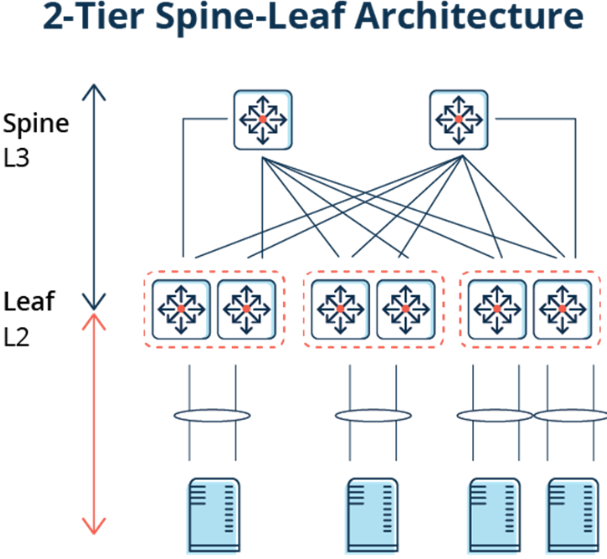
\includegraphics[width=0.7\linewidth]{image/16.png}
            \caption{Mô hình mạng 2-Tier (Spine-Leaf)}
            \label{fig:label1}
    \end{figure}
    
\begin{itemize}
    \item Mô hình mạng 2-Tier là một kiến trúc mạng hiện đại, giảm thiểu số lượng lớp trong mạng để tối ưu hóa hiệu suất và quản lý. Thay vì ba lớp (Core, Aggregation, Access) trong mô hình 3-Tier truyền thống, mạng 2-Tier chỉ gồm hai lớp: Spine và Leaf.
    \item Thường được sử dụng trong các trung tâm dữ liệu (Data Center) và các mạng doanh nghiệp vừa và nhỏ.
\end{itemize}

\subsubsection{Thành phần chính}
\begin{enumerate}
    \item \textbf{Leaf Layer (Tầng Leaf):}
    \begin{itemize}
        \item Tầng Leaf hoạt động như một lớp Access (truy cập), kết nối trực tiếp với các thiết bị đầu cuối như:
        \begin{itemize}
            \item Máy chủ (Servers).
            \item Các thiết bị lưu trữ (Storage).
            \item Máy tính cá nhân (Workstations) hoặc thiết bị mạng khác.
        \end{itemize}
        \item Tất cả các Switch Leaf đều kết nối trực tiếp với tất cả các Spine Switch, nhưng không kết nối trực tiếp với nhau.
    \end{itemize}

    \item \textbf{Spine Layer (Tầng Spine):}
    \begin{itemize}
        \item Tầng Spine hoạt động như lõi của mạng, chịu trách nhiệm chuyển tiếp lưu lượng giữa các Switch Leaf.
        \item Spine Switch không kết nối với thiết bị đầu cuối mà chỉ giao tiếp với các Switch Leaf.
        \item Cấu hình theo mô hình Full Mesh để đảm bảo mọi thiết bị trong hệ thống có thể giao tiếp với nhau qua nhiều đường dẫn.
    \end{itemize}
\end{enumerate}

\subsubsection{Nguyên lý hoạt động}
\begin{enumerate}
    \item \textbf{Non-Blocking Architecture (Kiến trúc không nghẽn):}
    \begin{itemize}
        \item Mỗi Switch Leaf kết nối trực tiếp với tất cả các Spine Switch, đảm bảo lưu lượng từ bất kỳ thiết bị nào cũng có nhiều đường dẫn để đến đích mà không bị nghẽn.
    \end{itemize}

    \item \textbf{Equal-Cost Multi-Path (ECMP):}
    \begin{itemize}
        \item Sử dụng nhiều đường dẫn có chi phí bằng nhau để tăng băng thông và giảm độ trễ.
        \item Hỗ trợ cân bằng tải giữa các kết nối Leaf và Spine, đảm bảo hiệu suất cao ngay cả khi có sự gia tăng lưu lượng.
    \end{itemize}

    \item \textbf{Redundancy (Dự phòng):}
    \begin{itemize}
        \item Các kết nối giữa Leaf và Spine được thiết kế dư thừa để giảm thiểu rủi ro mất kết nối khi xảy ra lỗi phần cứng.
    \end{itemize}
\end{enumerate}


\subsubsection{Ưu điểm}
\begin{enumerate}
    \item \textbf{Sắp xếp đơn giản: }Mô hình 2-Tier được thiết kế với cấu trúc đơn giản, trong đó các switch Leaf kết nối trực tiếp với các thiết bị đầu cuối như máy chủ và lưu trữ.

    \item \textbf{Chức năng Spine và Leaf: }Các switch Spine đảm bảo việc kết nối giữa tất cả các switch Leaf, tạo ra một mạng linh hoạt và hiệu quả.

    \item \textbf{Hiệu năng cao: }Giảm độ trễ (latency) và tăng tốc độ truyền tải dữ liệu nhờ kiến trúc kết nối trực tiếp và không nghẽn.

    \item \textbf{Khả năng mở rộng:}
    \begin{itemize}
        \item Dễ dàng mở rộng bằng cách thêm Leaf Switch (tăng thiết bị đầu cuối) hoặc Spine Switch (tăng khả năng xử lý lưu lượng).
        \item Không yêu cầu thay đổi cấu trúc tổng thể của mạng khi mở rộng.
    \end{itemize}

    \item \textbf{Đơn giản hóa quản lý:}
    \begin{itemize}
        \item Kiến trúc chỉ có hai tầng giúp việc cấu hình và quản lý mạng trở nên đơn giản hơn so với mô hình 3-Tier.
        \item Giảm số lượng giao thức phức tạp như STP (Spanning Tree Protocol).
    \end{itemize}

    \item \textbf{Tăng cường độ tin cậy: }Các kết nối dự phòng và tính năng ECMP giúp mạng hoạt động ổn định hơn ngay cả khi xảy ra sự cố.

    \item \textbf{Tối ưu hóa lưu lượng East-West: }Lưu lượng "East-West" (giữa các máy chủ trong cùng trung tâm dữ liệu) được tối ưu hóa, phù hợp với các ứng dụng hiện đại như Big Data, AI, và dịch vụ đám mây.
\end{enumerate}

\subsubsection{Hạn chế}
\begin{itemize}
    \item \textbf{Chi phí ban đầu: }Mặc dù giảm chi phí vận hành so với mô hình 3-Tier, nhưng việc triển khai mô hình 2-Tier ban đầu có thể yêu cầu các thiết bị hỗ trợ công nghệ hiện đại như Spine Switch có năng lực xử lý cao.
    \item \textbf{Quy mô giới hạn: }Đối với các hệ thống cực lớn (như doanh nghiệp toàn cầu hoặc trung tâm dữ liệu hyperscale), mô hình 2-Tier có thể gặp giới hạn về khả năng kết nối và quản lý lưu lượng.
\end{itemize}

\subsubsection{So sánh với mô hình 3-Tier}
\begin{table}[h!]
\centering
\begin{tabular}{|p{3cm}|p{5cm}|p{5cm}|}
\hline
\textbf{Tiêu chí} & \textbf{Mô hình 3-Tier} & \textbf{Mô hình 2-Tier (Spine-Leaf)} \\ 
\hline
Tầng kiến trúc & Access, Distribution, Core & Spine, Leaf \\ 
\hline
Độ phức tạp & Cao & Thấp \\ 
\hline
Khả năng mở rộng & Hạn chế, khó mở rộng linh hoạt & Dễ dàng mở rộng \\ 
\hline
Độ trễ (latency) & Cao (do nhiều tầng trung gian) & Thấp (kết nối trực tiếp Leaf-Spine) \\ 
\hline
Lưu lượng East-West & Chưa tối ưu & Tối ưu hóa tốt \\ 
\hline
Chi phí triển khai & Cao (nhiều tầng thiết bị) & Hợp lý (ít tầng hơn, tối ưu tài nguyên) \\ 
\hline
\end{tabular}
\caption{So sánh mô hình 3-Tier và 2-Tier (Spine-Leaf)}
\label{tab:comparison}
\end{table}

    \begin{figure}[h!]
        \centering
        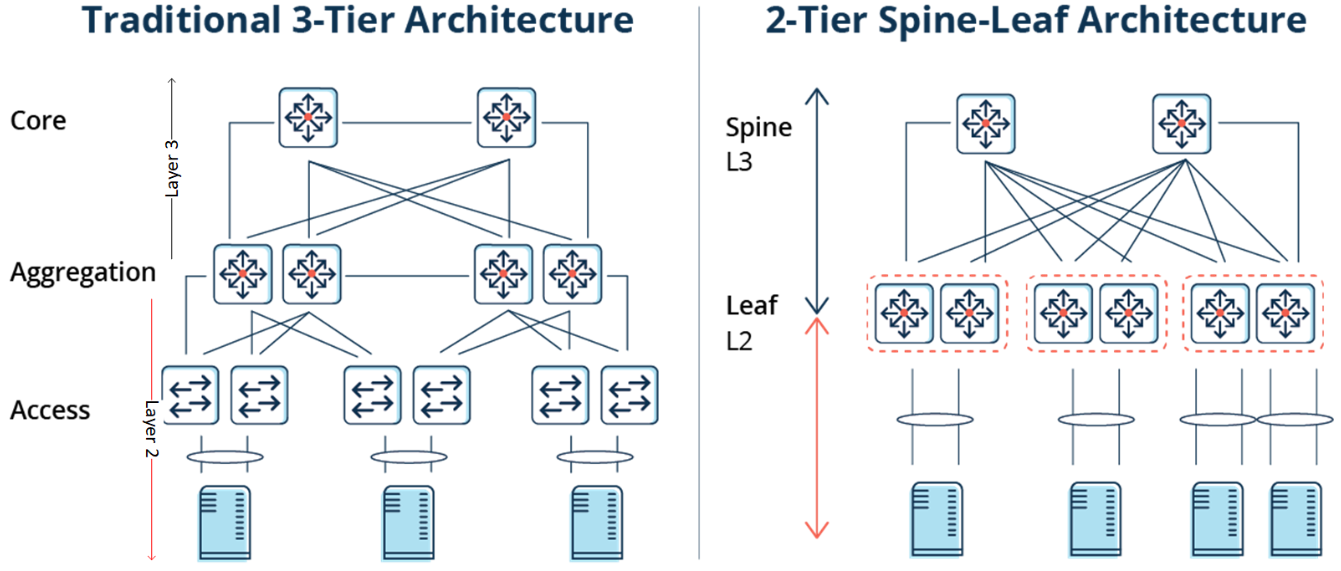
\includegraphics[width=0.7\linewidth]{image/17.png}
            \caption{So sánh mô hình 3-Tier và 2-Tier (Spine-Leaf)}
            \label{fig:label1}
    \end{figure}

\newpage
\subsubsection{Ứng dụng}
\begin{itemize}
    \item \textbf{Doanh nghiệp vừa và nhỏ: }Phù hợp cho các hệ thống yêu cầu kết nối đơn giản, nhanh chóng giữa các thiết bị.
    \item \textbf{Trung tâm dữ liệu: }Các trung tâm dữ liệu với lưu lượng trao đổi giữa các máy chủ nhiều hơn là giữa người dùng cuối và máy chủ.
    \item \textbf{Mạng doanh nghiệp: }Mô hình này lý tưởng cho các doanh nghiệp có yêu cầu mạng đơn giản và cần tối ưu chi phí triển khai.
\end{itemize}

\subsection{Tổng quan về DMZ (Demilitarized Zone)}
    \begin{figure}[h!]
        \centering
        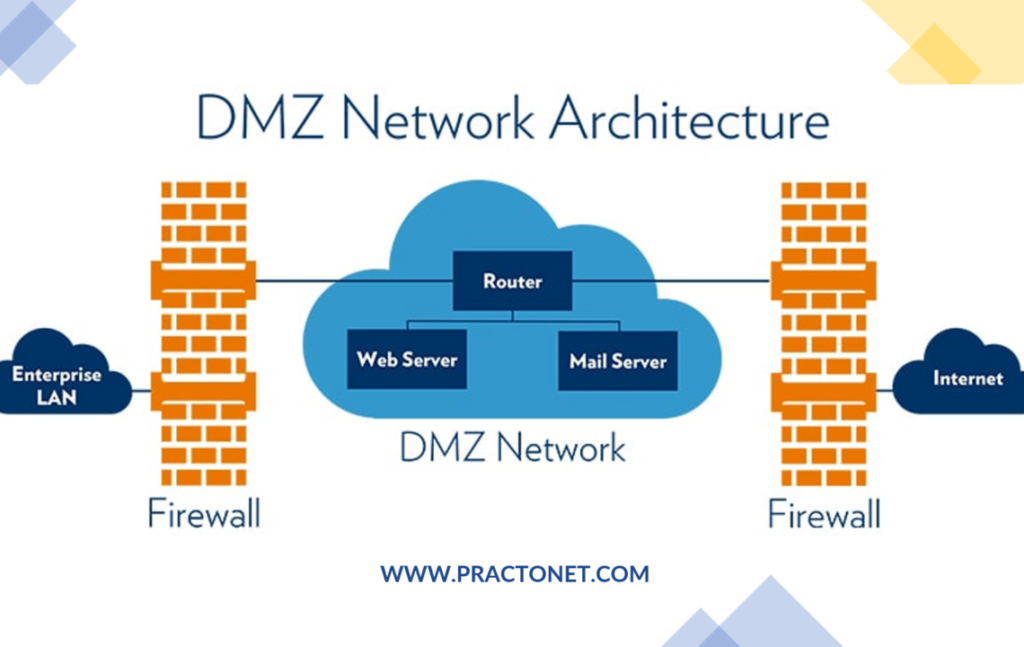
\includegraphics[width=0.7\linewidth]{image/18.png}
            \caption{DMZ (Demilitarized Zone)}
            \label{fig:label1}
    \end{figure}
    
\subsubsection{Khái niệm}
    DMZ (Demilitarized Zone) là một khu vực mạng được thiết kế để cô lập các tài nguyên hoặc dịch vụ công khai khỏi mạng nội bộ (Internal Network) và Internet. DMZ được triển khai nhằm giảm thiểu rủi ro tấn công mạng bằng cách giới hạn phạm vi truy cập vào các tài nguyên bên trong hệ thống mạng doanh nghiệp.

    Trong DMZ, các dịch vụ như máy chủ web, máy chủ DNS, máy chủ email hoặc VPN Gateway thường được đặt tại đây để người dùng bên ngoài có thể truy cập mà không ảnh hưởng đến mạng nội bộ.

\subsubsection{Mục đích của DMZ}
\begin{enumerate}
    \item \textbf{Tăng cường bảo mật:}
    \begin{itemize}
        \item DMZ ngăn chặn việc truy cập trực tiếp từ Internet vào mạng nội bộ, giảm nguy cơ rò rỉ thông tin hoặc tấn công.
        \item Bảo vệ mạng nội bộ khỏi các mối đe dọa bằng cách cô lập các tài nguyên công khai.
    \end{itemize}

    \item \textbf{Cô lập tài nguyên:}
    \begin{itemize}
        \item Các dịch vụ công khai được đặt trong DMZ để đảm bảo an toàn cho các hệ thống bên trong, ngay cả khi DMZ bị xâm nhập.
    \end{itemize}
    \item \textbf{Kiểm soát truy cập:}
    \begin{itemize}
        \item DMZ cho phép quản trị viên thiết lập các chính sách kiểm soát truy cập chặt chẽ giữa các vùng mạng, bao gồm mạng nội bộ, DMZ, và Internet.
    \end{itemize}
\end{enumerate}

\subsubsection{Cách triển khai DMZ}
\begin{enumerate}    
    \begin{itemize}
        \item \textbf{Thiết bị bảo mật:}
        \begin{itemize}
            \item Tường lửa (Firewall): Quản lý lưu lượng giữa mạng nội bộ, DMZ, và Internet.
            \item Bộ cân bằng tải (Load Balancer): Phân phối lưu lượng đến các máy chủ trong DMZ.
        \end{itemize}
        \item \textbf{Tài nguyên trong DMZ:}
        \begin{itemize}
            \item Máy chủ web (Web Server): Cung cấp dịch vụ trực tuyến như website hoặc API.
            \item Máy chủ DNS (Domain Name System): Giải quyết tên miền và cung cấp thông tin DNS cho người dùng bên ngoài.
            \item Máy chủ email (Mail Server): Xử lý email gửi và nhận từ bên ngoài.
            \item VPN Gateway: Cho phép kết nối từ xa an toàn vào mạng nội bộ qua DMZ.
        \end{itemize}
    \end{itemize}
    \item \textbf{Các phương pháp triển khai DMZ phổ biến:}
    \item \textbf{Cấu trúc cơ bản của DMZ:}
    \begin{figure}[h!]
        \centering
        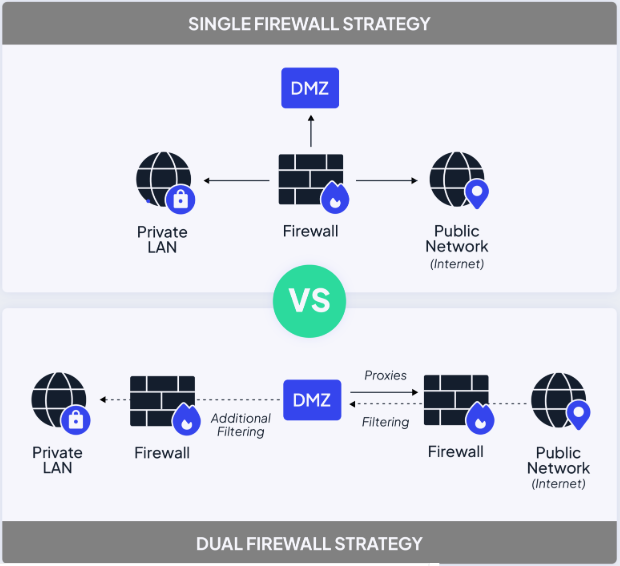
\includegraphics[width=0.7\linewidth]{image/19.png}
            \caption{Cấu trúc cơ bản của DMZ (Demilitarized Zone)}
            \label{fig:label1}
    \end{figure}
    
    \begin{enumerate}
        \item \textbf{Single Firewall DMZ (DMZ với một tường lửa):}
        \begin{itemize}
            \item Sử dụng một tường lửa với ba giao diện:
            \begin{itemize}
                \item Giao diện Internal (Nội bộ): Kết nối đến mạng nội bộ.
                \item Giao diện External (Bên ngoài): Kết nối đến Internet.
                \item Giao diện DMZ: Kết nối đến các tài nguyên trong khu vực DMZ.
            \end{itemize}
            \item Đây là cách triển khai đơn giản nhưng có độ bảo mật thấp hơn so với các mô hình khác.
        \end{itemize}
        
    \item \textbf{Dual Firewall DMZ (DMZ với hai tường lửa):}
    \begin{itemize}
        \item Sử dụng hai tường lửa:
        \begin{itemize}
            \item Tường lửa đầu tiên kiểm soát lưu lượng từ Internet vào DMZ.
            \item Tường lửa thứ hai kiểm soát lưu lượng từ DMZ vào mạng nội bộ.
        \end{itemize}
        \item Mô hình này tăng cường bảo mật bằng cách tạo hai lớp bảo vệ cho mạng nội bộ.  
    \end{itemize}
    
    \item \textbf{Cloud-based DMZ (DMZ trên nền tảng đám mây):}
    \begin{itemize}
        \item Sử dụng các dịch vụ bảo mật đám mây để triển khai DMZ, phù hợp với doanh nghiệp muốn tích hợp hệ thống mạng truyền thống và đám mây.
    \end{itemize}
    \end{enumerate}
\end{enumerate}

\subsubsection{Thành phần và nguyên tắc hoạt động}
\begin{enumerate}
    \item \textbf{Thành phần chính trong DMZ}
    \begin{itemize}
        \item \textbf{Firewall:}
        \begin{itemize}
            \item Thiết lập các chính sách kiểm soát lưu lượng ra vào DMZ.
            \item Lọc và kiểm tra lưu lượng đến từ Internet hoặc mạng nội bộ.
        \end{itemize}
        \item \textbf{Máy chủ (Servers):}
        \begin{itemize}
            \item Lưu trữ các dịch vụ công khai như web, email, hoặc DNS.
            \item Được cấu hình để chỉ cung cấp các dịch vụ cần thiết và hạn chế quyền truy cập.
        \end{itemize}
        \item \textbf{IDS/IPS (Intrusion Detection/Prevention Systems):}
        \begin{itemize}
            \item Giám sát lưu lượng mạng để phát hiện và ngăn chặn các cuộc tấn công.
        \end{itemize}
        \item \textbf{Load Balancer:}
        \begin{itemize}
            \item Phân phối lưu lượng truy cập đều đến các máy chủ trong DMZ, đảm bảo hiệu suất và tính sẵn sàng cao.
        \end{itemize}
    \end{itemize}

    \item \textbf{Nguyên tắc hoạt động của DMZ}
    \begin{itemize}
        \item \textbf{Kiểm soát lưu lượng:}
        \begin{itemize}
            \item Lưu lượng từ Internet được tường lửa kiểm tra và chỉ cho phép vào DMZ.
            \item DMZ chỉ cho phép lưu lượng hợp lệ đi vào mạng nội bộ thông qua tường lửa thứ hai (nếu có).
        \end{itemize}
        \item \textbf{Cô lập dịch vụ:}
        \begin{itemize}
            \item Các máy chủ trong DMZ được cô lập với mạng nội bộ, hạn chế khả năng lây nhiễm hoặc tấn công vào mạng chính.
        \end{itemize}
    \end{itemize}
\end{enumerate}

\subsubsection{Ưu điểm và hạn chế}
\begin{enumerate}
    \item \textbf{Ưu điểm}
    \begin{itemize}
        \item \textbf{Bảo mật cao:}
        \begin{itemize}
            \item Hạn chế quyền truy cập vào mạng nội bộ, giảm nguy cơ tấn công từ Internet.
            \item Tăng cường khả năng giám sát và kiểm soát lưu lượng mạng.
        \end{itemize}
        \item \textbf{Hỗ trợ hiệu quả cho các dịch vụ công khai: }Đảm bảo tính sẵn sàng và hiệu suất của các dịch vụ công khai như web hoặc email.
        \item \textbf{Dễ dàng quản lý: }Tài nguyên trong DMZ được quản lý độc lập, giảm tác động lên mạng nội bộ.
    \end{itemize}
    
    \item \textbf{Hạn chế}
    \begin{itemize}
        \item \textbf{Chi phí cao: }Đòi hỏi đầu tư vào tường lửa, thiết bị bảo mật, và máy chủ trong DMZ.
        \item \textbf{Phức tạp trong triển khai: }Yêu cầu cấu hình và quản lý chính xác để tránh lỗ hổng bảo mật.
        \item \textbf{Tài nguyên giới hạn: }DMZ thường chỉ chứa các dịch vụ công khai, không phù hợp để lưu trữ dữ liệu nhạy cảm.
    \end{itemize}
\end{enumerate}

\subsubsection{Ứng dụng thực tế}
\begin{enumerate}
    \item \textbf{Doanh nghiệp vừa và nhỏ: }DMZ được sử dụng để triển khai các dịch vụ như website, email, hoặc VPN mà không làm ảnh hưởng đến hệ thống nội bộ.

    \begin{figure}[h!]
        \centering
        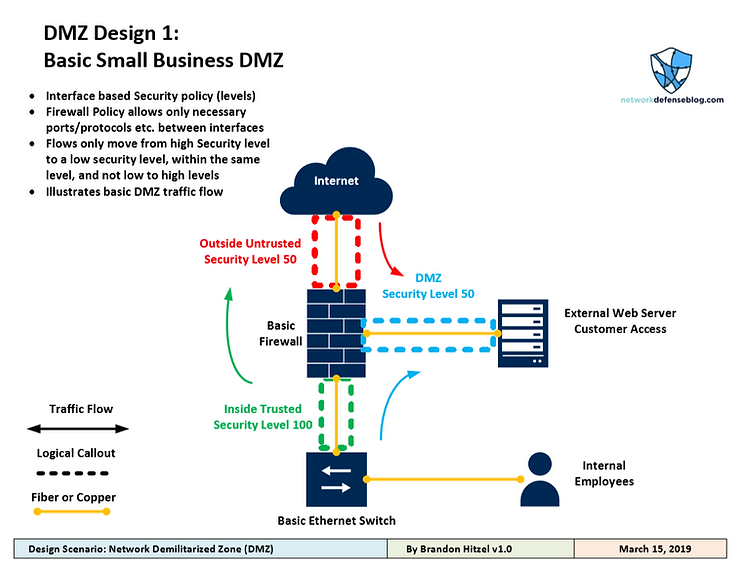
\includegraphics[width=0.7\linewidth]{image/20.png}
            \caption{Ứng dụng DZM cho mô hình doanh nghiệp nhỏ}
            \label{fig:label1}
    \end{figure}

    \begin{figure}[h!]
        \centering
        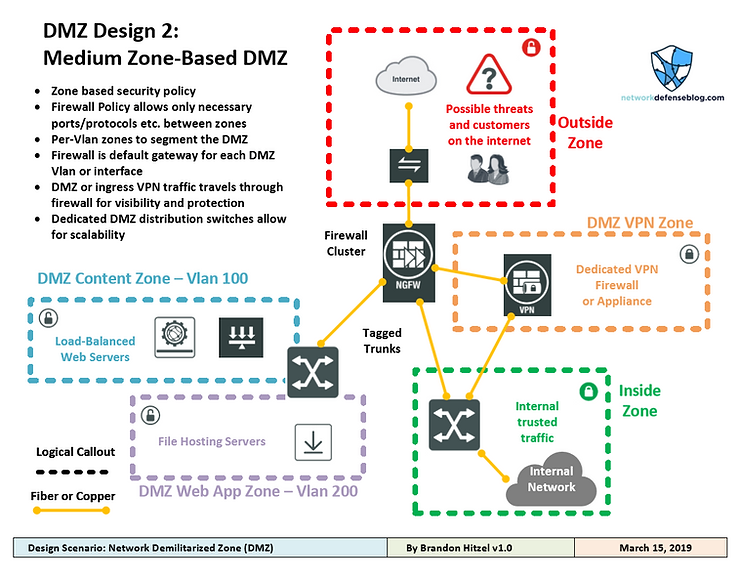
\includegraphics[width=0.7\linewidth]{image/21.png}
            \caption{Ứng dụng DZM cho mô hình doanh nghiệp vừa}
            \label{fig:label1}
    \end{figure}
    
    \item \textbf{Tổ chức lớn: }Kết hợp DMZ với các giải pháp bảo mật phức tạp hơn như IDS/IPS, tường lửa thế hệ mới (NGFW) để bảo vệ hệ thống toàn diện.

    \begin{figure}[h!]
        \centering
        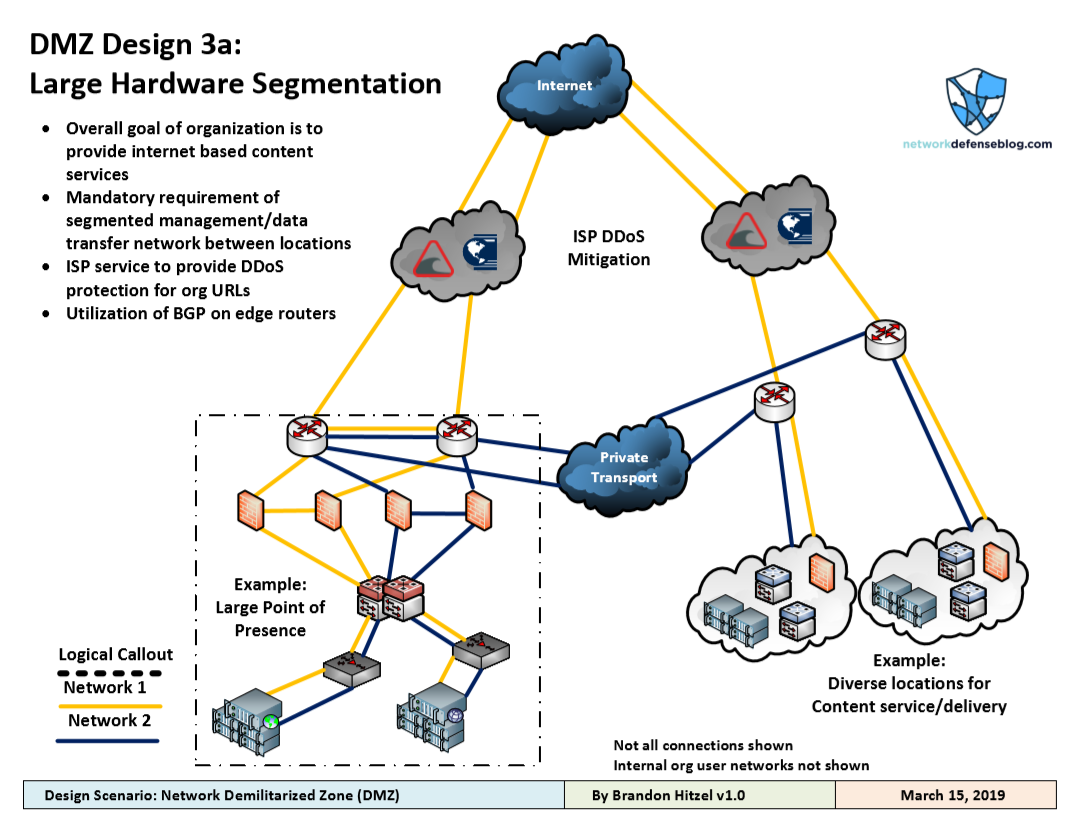
\includegraphics[width=0.7\linewidth]{image/22.png}
            \caption{Ứng dụng DZM cho mô hình tổ chức lớn}
            \label{fig:label1}
    \end{figure}
    
    \item \textbf{Trung tâm dữ liệu: }DMZ giúp cô lập và bảo vệ các dịch vụ đám mây, API, và tài nguyên công khai khỏi các cuộc tấn công mạng.
\end{enumerate}

\subsection{Phần mềm EVE-NG}
\subsubsection{Giới thiệu EVE-NG}
EVE-NG là một phần mềm hỗ trợ mô phỏng mạng. Phần mềm này cung cấp khả năng thiết lập và mô phỏng các mạng ảo bằng cách sử dụng nhiều loại máy ảo (VM) và thiết bị mạng đa dạng. EVE-NG hướng đến các chuyên gia mạng, sinh viên ngành CNTT, và các giảng viên cần mô phỏng các kịch bản mạng phức tạp để phục vụ mục đích thử nghiệm, giảng dạy, và chuẩn bị cho các kỳ thi chứng chỉ.\\

    \begin{figure}[h!]
        \centering
        
\includegraphics[width=0.7\linewidth]{image/23.png}
            \caption{Phần mềm EVE-NG}
            \label{fig:label1}
    \end{figure}

Phần mềm này có giao diện đồ họa thân thiện và dễ sử dụng, cho phép người dùng xây dựng các cấu trúc liên kết mạng ảo và vận hành các thiết bị trong môi trường mô phỏng. Nền tảng EVE-NG cũng tích hợp các mô-đun dịch vụ mạng, giúp người dùng có thể thêm các máy chủ ảo như máy chủ DHCP, máy chủ DNS, và
máy chủ web vào các mạng ảo.

EVE-NG có khả năng hoạt động trên máy tính cục bộ hoặc máy chủ từ xa, đồng thời hỗ trợ nhiều hệ thống ảo hóa như VMware ESXi, VirtualBox, và KVM. Phần mềm này còn cung cấp một API mạnh mẽ, giúp người dùng có thể tự động hóa các tác vụ cấu hình và triển khai mạng bằng các ngôn ngữ lập trình kịch bản như Python.(Harahus et al., 2023)

\subsubsection{Ưu, nhược điểm của EVE-NG}
\begin{enumerate}
    \item \textbf{Ưu điểm}
    \begin{itemize}
        \item EVE-NG cung cấp giao diện đồ họa trực quan qua trình duyệt web, giúp việc truy cập và quản lý các mô phỏng mạng trở nên đơn giản hơn. Người dùng có thể dễ dàng thiết lập và cấu hình các node mạng từ thư viện mẫu, kết nối chúng và theo dõi hoạt động mạng một cách trực quan. Điều này tiết kiệm đáng kể thời gian và công sức so với việc cấu hình thủ công từng thiết bị.
        \item EVE-NG hỗ trợ một loạt các thiết bị mạng và hệ thống ảo hóa khác nhau. Người dùng có thể sử dụng Dynamips, IOU, cũng như các thiết bị mã nguồn mở như router trên QEMU để mô phỏng các mạng từ đơn giản đến phức tạp. Tính năng này giúp kiểm tra và đánh giá hiệu suất mạng trước khi triển khai thực tế.
        \item Quản trị viên và người dùng có kinh nghiệm có thể thêm image phần mềm vào thư viện để tạo ra các thiết bị mạng tùy chỉnh. Điều này cho phép xây dựng các mô hình lab phức tạp, đáp ứng linh hoạt nhu cầu đào tạo, kiểm thử và nghiên cứu. Tính năng này đặc biệt hữu ích cho các tổ chức đào tạo và trung tâm nghiên cứu, giúp dễ dàng tạo ra các kịch bản mạng phong phú và chính xác.
        \item EVE-NG là một dự án mã nguồn mở, được phát triển và duy trì bởi cộng đồng trên GitLab. Sự đóng góp từ người dùng và các nhà phát triển giúp công cụ này liên tục được cải thiện, đảm bảo tính ổn định và cập nhật các tính năng mới. Cộng đồng đóng góp này cũng giúp EVE-NG trở nên đáng tin cậy và linh hoạt, đáp ứng nhu cầu đa dạng của người dùng.
        \item EVE-NG có khả năng hỗ trợ nhiều hypervisors trên một máy ảo, giúp tích hợp và quản lý các môi trường ảo hóa khác nhau. Điều này cho phép tối ưu hóa tài nguyên hệ thống và cải thiện hiệu suất của các mô phỏng mạng. Người dùng có thể dễ dàng chuyển đổi giữa các môi trường ảo hóa, nâng cao khả năng quản lý và vận hành mạng mà không gặp trở ngại.
    \end{itemize}

    \item \textbf{Nhược điểm}
    \begin{itemize}
        \item Để chạy các mô hình mạng phức tạp và nhiều thiết bị ảo, EVE-NG yêu cầu một hệ thống phần cứng mạnh mẽ với nhiều tài nguyên CPU, RAM và dung lượng ổ đĩa. Điều này có thể là một thách thức đối với các cá nhân hoặc tổ chức không có điều kiện đầu tư vào phần cứng cao cấp. Việc nâng cấp và duy trì phần cứng để đáp ứng yêu cầu của EVE-NG cũng có thể tốn kém.
        \item Việc cài đặt và cấu hình EVE-NG ban đầu có thể phức tạp, đặc biệt đối với những người dùng mới hoặc không có nhiều kinh nghiệm về hệ thống mạng và ảo hóa. Quá trình này đòi hỏi kiến thức về các công cụ ảo hóa, hệ điều hành Linux và các công nghệ mạng liên quan. Người dùng cần phải nắm vững các bước cấu hình cơ bản và biết cách xử lý các sự cố phát sinh trong quá trình cài đặt.
        \item Mặc dù EVE-NG có một cộng đồng người dùng tích cực, việc tìm kiếm hỗ trợ kỹ thuật chuyên sâu có thể gặp khó khăn. Người dùng có thể phải dựa vào các tài liệu và diễn đàn cộng đồng để giải quyết các vấn đề phát sinh, điều này không phải lúc nào cũng đảm bảo được sự hỗ trợ nhanh chóng và hiệu quả.
        \item Một số hình ảnh phần mềm và thiết bị có thể không tương thích hoàn toàn với EVE-NG, dẫn đến các vấn đề về hiệu suất hoặc tính năng. Việc tìm kiếm và cấu hình các image tương thích có thể tốn thời gian và công sức, đặc biệt đối với các thiết bị hoặc phần mềm ít phổ biến.
    \end{itemize}
\end{enumerate}

\newpage
\renewcommand{\thesubsection}{\thesection.\arabic{subsection}} % Đặt lại số của subsection từ 1 mỗi section mới
\setcounter{section}{3} % Đặt số thứ tự cho section
\setcounter{subsection}{0}
\section*{CHƯƠNG 3 - PHÂN TÍCH VÀ THIẾT KẾ HỆ THỐNG}
\addcontentsline{toc}{section}{CHƯƠNG 3 - PHÂN TÍCH VÀ THIẾT KẾ HỆ THỐNG}
\subsection{Khảo sát yêu cầu của doanh nghiệp}
\subsubsection{Tổng quan về nhu cầu doanh nghiệp}
\begin{itemize}
    \item \textbf{Loại hình doanh nghiệp: }Doanh nghiệp vừa và nhỏ, hoạt động trong lĩnh vực cung cấp dịch vụ và thương mại.
    \item \textbf{Yêu cầu chính:}
    \begin{itemize}
        \item Xây dựng một hệ thống mạng hiện đại, đảm bảo tính bảo mật và khả năng mở rộng.
        \item Hỗ trợ các dịch vụ công cộng (web, email) và nội bộ (chia sẻ tài liệu, quản lý nhân sự).
        \item Tích hợp khu vực DMZ để đảm bảo cô lập dịch vụ công cộng và bảo vệ hệ thống nội bộ.
        \item Hỗ trợ kết nối chi nhánh từ xa thông qua VPN.
        \item Đảm bảo hiệu suất cao với việc sử dụng VXLAN và mô hình mạng 2-tier.
    \end{itemize}
\end{itemize}

\subsubsection{Các yêu cầu cụ thể}
Doanh nghiệp yêu cầu thiết kế một hệ thống mạng với các tiêu chí cụ thể sau:
\begin{enumerate}
    \item \textbf{Kết nối mạng LAN: }Tất cả các máy tính để bàn (PC) của nhân viên các bộ phận cần được kết nối trong một mạng cục bộ (LAN).

    \item \textbf{Truy cập internet:}
    \begin{itemize}
        \item Đảm bảo tất cả PC trong mạng có khả năng truy cập internet.
        \item Cần áp dụng các quy định để hạn chế nhân viên truy cập các trang web không phù hợp.
    \end{itemize}


    \item \textbf{Hiệu suất mạng: }
    \begin{itemize}
        \item Đảm bảo băng thông và độ trễ thấp cho các ứng dụng quan trọng như quản lý dữ liệu và hội thoại video.
    \end{itemize}

    \item \textbf{Bảo mật:}
    \begin{itemize}
        \item Thiết lập DMZ để bảo vệ các dịch vụ công cộng như máy chủ email và file.
        \item Đảm bảo kết nối an toàn, ngăn chặn truy cập trái phép vào mạng nội bộ.
    \end{itemize}

    \item \textbf{Khả năng mở rộng: }Dễ dàng mở rộng khi doanh nghiệp tăng số lượng chi nhánh hoặc người dùng.

    \item \textbf{Khả năng quản lý: }Đơn giản hóa việc quản lý và giám sát hệ thống mạng, sử dụng giao diện quản trị tập trung.

    \item \textbf{Hỗ trợ chi nhánh: }Kết nối chi nhánh từ xa thông qua ISSEC VPN Tunnel, đảm bảo tính liên tục và bảo mật.
\end{enumerate}

\subsection{Phạm vi của hệ thống}
\subsubsection{Quy mô của hệ thống:}
\begin{itemize}
    \item \textbf{Số lượng người dùng:}
    \begin{itemize}
        \item Trụ sở chính: Khoảng 50-100 nhân viên.
        \item Chi nhánh: Khoảng 20-30 nhân viên.
    \end{itemize}
    \item \textbf{Thiết bị chính:}
    \begin{itemize}
        \item Máy chủ tại khu vực DMZ: 3 máy chủ (Mail Server, File Server, Backup Server).
        \begin{itemize}
            \item Hai máy chủ trung tâm để lưu trữ dữ liệu nhân viên (File Server và Backup Sever) và quản lý dịch vụ in ấn.
            \item Một máy chủ email để cung cấp tài khoản email cho các nhân viên của các phòng ban khác nhau.
        \end{itemize}
        \item \textbf{Thiết bị mạng:}
        \begin{itemize}
            \item Tường lửa ASA.
            \item Switch Layer 2, Layer 3.
            \item Router kết nối VPN.
            \item Hệ thống Wi-Fi Controller (WLC) cho các điểm truy cập không dây.
            \item Máy in đặt tại mỗi văn phòng.
        \end{itemize}
        \item \textbf{Khu vực mạng:}
        \begin{itemize}
            \item Mạng nội bộ (LAN): Kết nối các phòng ban và các khu vực trong doanh nghiệp.
            \item DMZ: Triển khai máy chủ Email, File, và Backup để bảo vệ dữ liệu nội bộ.
            \item Kết nối VPN: Kết nối an toàn giữa các chi nhánh hoặc giữa nhân viên từ xa và hệ thống trung tâm.
        \end{itemize}
    \end{itemize}
\end{itemize}

\subsubsection{Mô hình mạng:}
\begin{enumerate}
    \item \textbf{Kiến trúc mạng:}
    \begin{itemize}
        \item Mô hình 2-tier: Bao gồm Spine và Leaf, đảm bảo hiệu suất cao và giảm độ phức tạp, với cấu trúc bao gồm:
        \begin{itemize}
            \item Lớp Spine: Đảm nhận vai trò truyền tải dữ liệu giữa các thiết bị Leaf với tốc độ cao.
            \item Lớp Leaf: Kết nối trực tiếp đến các máy tính để bàn và máy in.
        \end{itemize}
        \item Sử dụng VXLAN để cải thiện khả năng mở rộng và phân đoạn mạng ảo.
    \end{itemize}
    
    \item \textbf{Khu vực mạng:}
    \begin{itemize}
        \item \textbf{DMZ (Demilitarized Zone): }Chứa các tài nguyên công cộng như máy chủ Mail, File, và Backup.
        \item \textbf{Mạng nội bộ: }Kết nối các máy trạm, thiết bị mạng và các tài nguyên nội bộ.
        \item \textbf{Mạng chi nhánh: }Kết nối từ xa thông qua VPN Tunnel, đảm bảo bảo mật và độ tin cậy.
    \end{itemize}
\end{enumerate}

\subsubsection{Phân chia VLAN:}
Mô hình bao gồm 1 trụ sở chính và 1 chi nhánh. Trong đó trụ sở chính có 5 VLAN được thiết kế để phân vùng mạng, cụ thể:
\begin{itemize}
    \item \textbf{VLAN 10 - Sale:}
    \begin{itemize}
        \item Kết nối các máy trạm thuộc phòng nhân sự (HR-PC01).
        \item Đảm bảo bảo mật cao cho dữ liệu nhạy cảm.
    \end{itemize}

    \item \textbf{VLAN 20 - FIN (Finance):}
    \begin{itemize}
        \item Kết nối các máy trạm của phòng tài chính (FINANCE-PC01).
        \item Cần ưu tiên băng thông và độ bảo mật để xử lý dữ liệu tài chính.
    \end{itemize}
    
    \item \textbf{VLAN 30 - HR (Human Resources):}
    \begin{itemize}
        \item Phục vụ cho các máy trạm của phòng kinh doanh (SALE-PC01).
        \item Cần đảm bảo tính ổn định để sử dụng các ứng dụng giao tiếp.
    \end{itemize}

    \item \textbf{VLAN 40 - MAR (Marketing):}
    \begin{itemize}
        \item Kết nối các thiết bị của phòng marketing (MARETING-PC01).
        \item Cần băng thông trung bình để truy cập tài nguyên chia sẻ.
    \end{itemize}
    
    \item \textbf{VLAN 50 - IT:}
    \begin{itemize}
        \item Dành cho phòng IT (IT-PC01) và quản lý thiết bị mạng.
        \item Có quyền truy cập vào mọi VLAN khác để hỗ trợ và quản trị.
    \end{itemize}
\end{itemize}

Chi nhánh gồm 2 VLAN được thiết kế như sau:
\begin{itemize}
    \item \textbf{VLAN 11 - PROD (Products)}
        \begin{itemize}
            \item Phục vụ cho các máy trạm tại phòng sản xuất (PROD-PC01).
            \item Cần đảm bảo tính ổn định và bảo mật cho nhu cầu sản xuất sản phẩm.
        \end{itemize}
    \item \textbf{VLAN 21 - SUPPLY}
        \begin{itemize}
            \item Phục vụ cho các máy trạm tại phòng cung ứng (SUPPLY-PC01).
            \item Cần băng thông trung bình và tính sẵn sàng.
        \end{itemize}
\end{itemize}
\subsection{Phân tích chi tiết hệ thống mạng}
\subsubsection{Băng thông hệ thống:}
\begin{enumerate}
    \item \textbf{Kết nối Spine - Leaf (Port-Channel):}
    \begin{itemize}
        \item Sử dụng các đường truyền 10Gbps giữa các switch Spine và Leaf để đảm bảo lưu lượng lớn và tối ưu hiệu suất.
        \item Cấu hình Port-Channel (EtherChannel) giữa các Spine để tăng dung lượng băng thông và dự phòng kết nối.
    \end{itemize}
    \item \textbf{Kết nối Leaf - Thiết bị cuối:}
    \begin{itemize}
        \item Máy tính để bàn và máy in được kết nối qua các cổng Ethernet 1Gbps.
        \item Truyền tải dữ liệu nhanh giữa các máy tính thuộc cùng VLAN.
        \item Đảm bảo mỗi Leaf Switch hỗ trợ ít nhất 24 cổng Ethernet, đáp ứng nhu cầu mở rộng trong tương lai.
    \end{itemize}
    \item \textbf{Kết nối tới DMZ:}
    \begin{itemize}
        \item Tốc độ:
        \begin{itemize}
            \item Từ ASA tới switch: 1 Gbps.
            \item Từ switch tới các máy chủ: 1 Gbps.
        \end{itemize}
        \item Đảm bảo: Đủ băng thông để xử lý truy cập từ bên ngoài tới các dịch vụ công cộng (Email, File).
    \end{itemize}

    \item \textbf{Kết nối VPN (ISSEC VPN Tunnel):}
    \begin{itemize}
        \item Từ ISP01/ISP02 tới các chi nhánh:
        \begin{itemize}
            \item Tốc độ tối thiểu 100 Mbps cho mỗi đường truyền.
            \item Sử dụng VPN mã hóa để bảo vệ dữ liệu trong quá trình truyền tải.
        \end{itemize}
        \item Ưu tiên băng thông: Phòng tài chính và nhân sự sẽ được ưu tiên băng thông qua cơ chế QoS.
    \end{itemize}

    \item \textbf{Tổng kết:}
    \begin{itemize}
        \item Số lượng kết nối:
        \begin{itemize}
            \item Spine-Leaf: 6 kết nối 10 Gbps.
            \item Leaf-End devices: Hơn 10 kết nối 1 Gbps.
        \end{itemize}
        \item Dung lượng băng thông tổng:
        \begin{itemize}
            \item Spine-Leaf: 60 Gbps (tổng cộng 6 liên kết).
            \item Hỗ trợ tối đa hơn 200 máy trạm trong tương lai mà không gây ra nghẽn mạng.
        \end{itemize}
    \end{itemize}
\end{enumerate}

\subsubsection{Khu vực DMZ:}
\begin{itemize}
    \item DMZ (Demilitarized Zone) được thiết kế để cô lập các dịch vụ công cộng khỏi mạng nội bộ, gồm:
        \begin{itemize}
        \item \textbf{Máy chủ Mail: }Xử lý thư điện tử công ty.
        \item \textbf{Máy chủ File: }Chia sẻ tài liệu với người dùng bên ngoài.
        \item \textbf{Máy chủ Backup: }Lưu trữ và bảo vệ dữ liệu quan trọng.
        \end{itemize}
    \item Các thiết bị trong DMZ được cách ly với mạng nội bộ thông qua tường lửa (ASA), giúp ngăn chặn truy cập trái phép.
\end{itemize}

\begin{itemize}
    \item \textbf{Chức năng:}
    \begin{itemize}
        \item Lưu trữ các máy chủ dịch vụ như Mail Server, File Server, và Backup Server.
        \item Đảm bảo tính bảo mật bằng cách cách ly các tài nguyên công cộng khỏi mạng nội bộ.
    \end{itemize}
    
    \item \textbf{Triển khai:}
    \begin{itemize}
        \item Cấu hình hai Firewall ASA hoạt động trong chế độ High Availability (HA).
        \item Cấp quyền truy cập hạn chế đến DMZ từ Internet thông qua các chính sách tường lửa.
    \end{itemize}
\end{itemize}

\subsubsection{Hiệu suất và bảo mật:}
\begin{itemize}
    \item \textbf{VPN: }Thiết lập kết nối VPN an toàn giữa các chi nhánh hoặc giữa nhân viên từ xa và hệ thống trung tâm.
\end{itemize}

\subsubsection{Giám sát và quản lý mạng:}
\begin{itemize}
    \item Giám sát hiệu suất mạng: Sử dụng các công cụ giám sát để theo dõi hiệu suất của hệ thống mạng.
    \item Quản lý truy cập: Đảm bảo rằng chỉ những người dùng có thẩm quyền mới có thể truy cập vào các tài nguyên mạng.
\end{itemize}

\subsubsection{Bảo trì hệ thống:}
\begin{itemize}
    \item Kiểm tra và cập nhật: Thường xuyên kiểm tra và cập nhật các thiết bị mạng và phần mềm để đảm bảo hệ thống luôn hoạt động hiệu quả.
    \item Xử lý sự cố: Nhanh chóng xử lý các sự cố mạng để đảm bảo tính liên tục của hoạt động kinh doanh.
\end{itemize}

\subsubsection{Đánh giá và cải thiện:}
\begin{itemize}
    \item Đánh giá hiệu quả: Đánh giá hiệu quả của hệ thống mạng mới sau khi triển khai.
    \item Đưa ra các cải tiến: Dựa trên kết quả đánh giá, đề xuất các cải tiến để nâng cao hiệu suất và bảo mật của hệ thống mạng trong tương lai.
\end{itemize}

\subsection{Tổng kết về mô hình}
\begin{itemize}
    \item Mô hình 2-Tier với 2 cơ sở (trụ sở chính và chi nhánh). Trong đó, 5 VLAN tại trụ sở chính, 2 VLAN tại chi nhánh và khu vực DMZ gồm các Sever.
    \item Tích hợp thêm hệ thống tường lửa để đảm bảo khả năng bảo mật, ngăn chặn các truy cập trái phép từ bên ngoài. \item Đồng thời triển khai kết nối VPN, kết nối an toàn giữa các chi nhánh hoặc giữa nhân viên từ xa và hệ thống trung tâm.
    \item Băng thông cao (10 Gbps ở Spine-Leaf, 1 Gbps ở thiết bị đầu cuối) đảm bảo đáp ứng nhu cầu sử dụng hiện tại và tương lai.
    \item Hệ thống mạng này phù hợp với doanh nghiệp vừa và nhỏ, hỗ trợ đầy đủ tính năng và bảo mật cần thiết cho hoạt động hàng ngày.
\end{itemize}

\subsection{ Thiết kế mô hình mạng}
\subsubsection{Sơ đồ vật lý}
    \begin{figure}[h!]
        \centering
        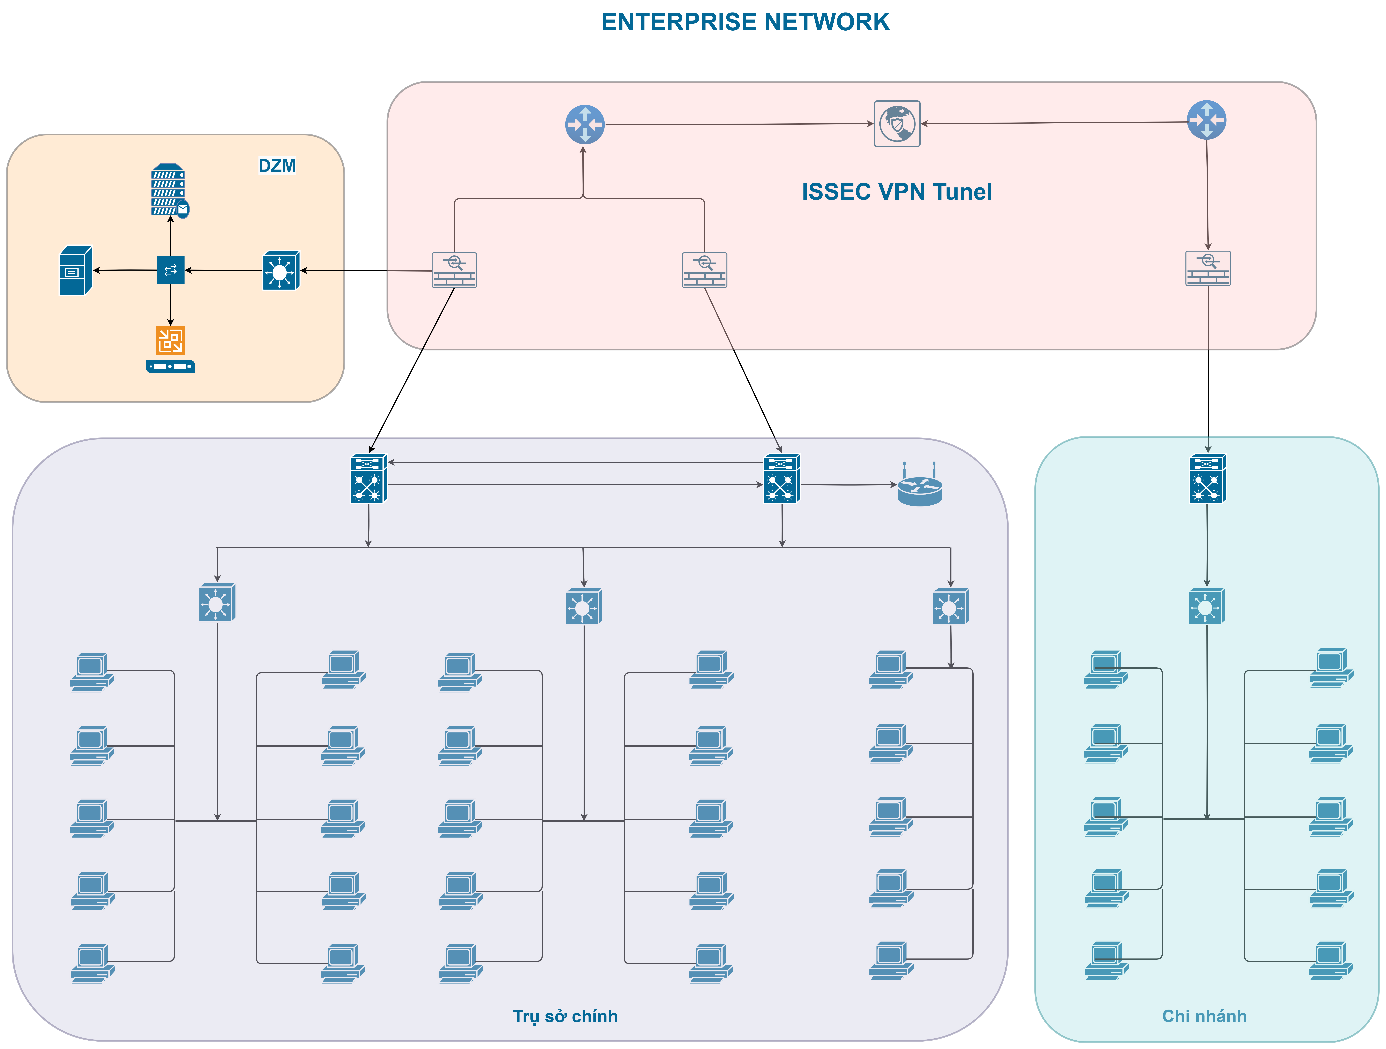
\includegraphics[width=1
        \linewidth]{image/24.png}
            \caption{Sơ đồ vật lý}
            \label{fig:label1}
    \end{figure}

\newpage
\subsubsection{Sơ đồ logic}
    \begin{figure}[h!]
        \centering
        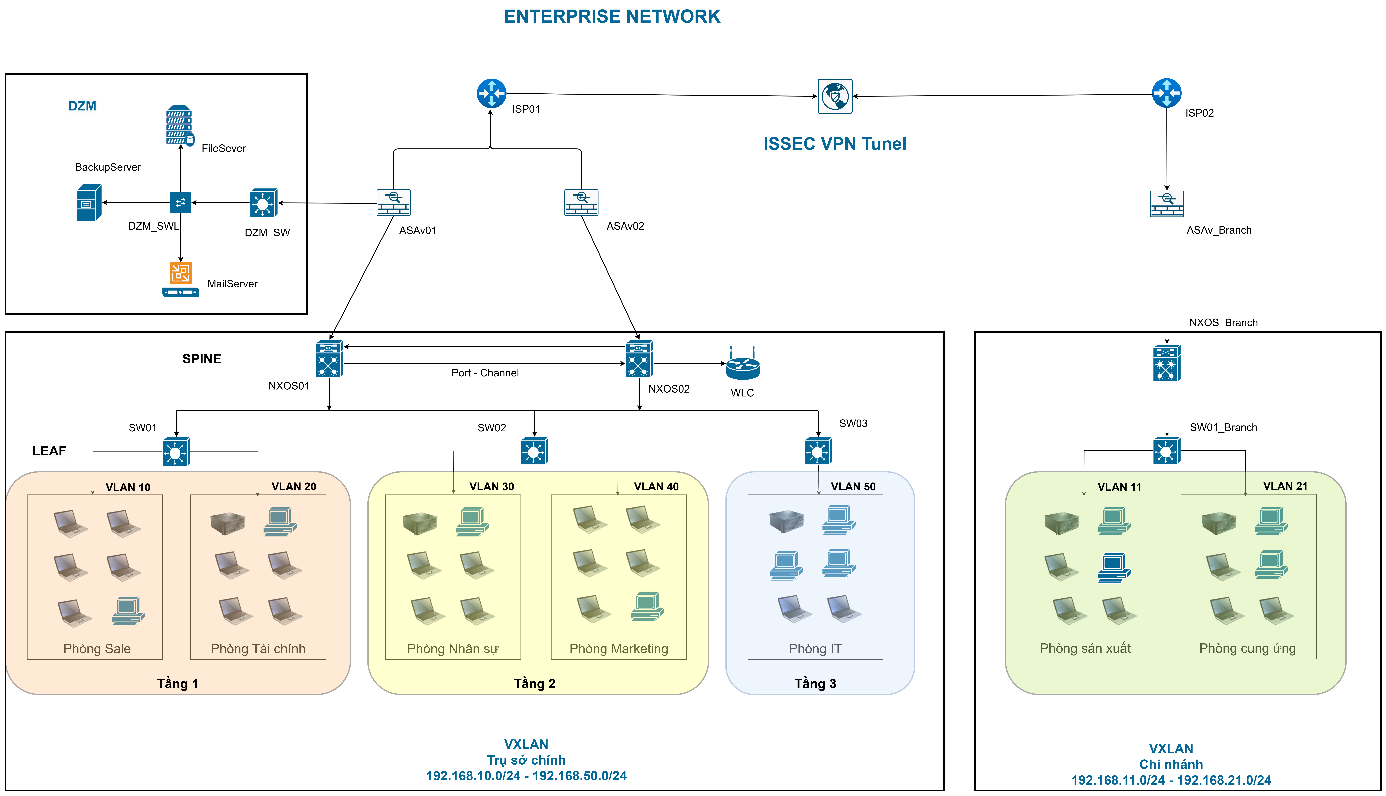
\includegraphics[width=1
        \linewidth]{image/25.png}
            \caption{Sơ đồ logic}
            \label{fig:label1}
    \end{figure}


\newpage
\subsubsection{Sơ đồ luận lý}
    \begin{figure}[h!]
        \centering
        \includegraphics[width=1
        \linewidth]{image/26.png}
            \caption{Sơ đồ luận lý}
            \label{fig:label1}
    \end{figure}


\subsubsection{Thông tin cài đặt cấu hình hệ thống}

\begin{enumerate}
\item \textbf{Thông tin các thiết bị trong hệ thống}


\begin{table}[h!]
\centering
\begin{tabular}{|p{2cm}|p{5cm}|p{7cm}|}
\hline
\textbf{Tên loại thiết bị} & \textbf{Tên của thiết bị} & \textbf{Mô tả thiết bị} \\ 
\hline
\multicolumn{3}{|c|}{\textbf{Trụ sở chính}} \\ 
\hline
Router & ISP01 & Đảm bảo kết nối giữa mạng chính và mạng tại các chi nhánh thông qua một đường hầm VPN IPsec an toàn. \\ 
\hline
Firewall ASAv & ASAv01, ASAv02 & Chịu trách nhiệm bảo vệ DMZ bằng cách kiểm soát và lọc lưu lượng giữa DMZ và mạng bên ngoài. ASA01 và ASA02 cũng kết nối với router ISP01 để tạo kết nối Internet an toàn, đồng thời duy trì thông tin phân vùng mạng và các chính sách bảo mật. \\ 
\hline
Cisco Nexus 9000v & NXOS01, NXOS02 & Chịu trách nhiệm định tuyến lưu lượng giữa các switch leaf và đảm bảo sự ổn định của toàn bộ mạng. \\ 
\hline
Switch layer 3 & SW01, SW02, SW03 & Chịu trách nhiệm kết nối trực tiếp với các máy trạm ở các phòng ban khác nhau như phòng Sale, phòng Finance, phòng Human Resource, phòng Kỹ thuất và phòng Marketing. \\ 
\hline
\end{tabular}
\caption{Thông tin các thiết bị trong hệ thống (1)}
\label{tab:comparison}
\end{table}


\begin{table}[h!]
\centering
\begin{tabular}{|p{2cm}|p{5cm}|p{7cm}|}
\hline
\textbf{Tên loại thiết bị} & \textbf{Tên của thiết bị} & \textbf{Mô tả thiết bị} \\ 
\hline
\multicolumn{3}{|c|}{\textbf{Khu vực DMZ}} \\ 
\hline
Switch layer 3 & DMZ-SW & Quản lý luồng dữ liệu giữa các thiết bị trong khu vực DMZ, đồng thời kết nối với các firewall ASA01 và ASA02. \\ 
\hline
Switch layer 2 & DMZ-SWL2 & Quản lý luồng dữ liệu giữa các thiết bị trong khu vực DMZ, đồng thời kết nối với các firewall ASA01 và ASA02.\\
\hline
Server & WinServer & Chịu trách nhiệm cung cấp các dịch vụ như mail server, web server, ftp server, đảm bảo an toàn nhờ kết nối với DMZ-SWL2.\\
\hline
\end{tabular}
\caption{Thông tin các thiết bị trong hệ thống (2)}
\label{tab:comparison}
\end{table}

\begin{table}[h!]
\centering
\begin{tabular}{|p{2cm}|p{5cm}|p{7cm}|}
\hline
\textbf{Tên loại thiết bị} & \textbf{Tên của thiết bị} & \textbf{Mô tả thiết bị} \\ 
\hline
\multicolumn{3}{|c|}{\textbf{Chi nhánh}} \\ 
\hline
Router & ISP02 & Đảm bảo kết nối giữa mạng chính và mạng tại các chi nhánh thông qua một đường hầm VPN IPsec an toàn.\\
\hline
Firewall ASAv & ASAv-Branch & Chịu trách nhiệm bảo vệ và kiểm soát lưu lượng dữ liệu đến và đi.\\
\hline
Cisco Nexus 9000v & NXOS-Branch & Quản lý luồng dữ liệu từ các thiết bị tại chi nhánh và kết nối với switch leaf SW01-Branch.\\
\hline
Switch layer 3 & SW01-Branch & Nơi kết nối trực tiếp với các máy trạm thuộc các bộ phận như phòng Sản xuất và phòng Cung ứng tại chi nhánh. Điều này đảm bảo khả năng phân đoạn và bảo mật dữ liệu giữa chi nhánh và mạng chính.\\
\hline
\end{tabular}
\caption{Thông tin các thiết bị trong hệ thống}
\label{tab:comparison}
\end{table}


\item \textbf{Thông tin VLAN, VXLAN của hệ thống}
\begin{table}[h!]
\centering
\begin{tabular}{|p{2cm}|p{2cm}|p{2cm}|p{2.5cm}|p{2.5cm}|p{2.5cm}|}
\hline
\textbf{Tên VLAN} & \textbf{VLANID} & \textbf{VXLAN ID} & \textbf{Mô tả} & \textbf{Subnet} & \textbf{Default Gateway}\\ 
\hline
\multicolumn{6}{|c|}{\textbf{Trụ sở chính}} \\ 
\hline
Phòng Sale & 10 & 10010 & Vlan cho thiết bị của phòng Sale & 192.168.10.0/24 & 192.168.10.1\\
\hline
Phòng Tài chính & 20 & 10020 & Vlan cho thiết bị phòng Tài chính & 192.168.20.0/24 & 192.168.20.1\\
\hline
Phòng Nhân sự & 30 & 10030 & Vlan cho thiết bị phòng Nhân sự & 192.168.30.0/24 & 192.168.30.1 \\
\hline
Phòng Marketing & 40 & 10040 & Vlan cho thiết bị phòng Marketing & 192.168.40.0/24 & 192.168.40.1\\
\hline
Phòng hỗ trợ kỹ thuật & 50 & 10050 & Vlan cho thiết bị phòng hỗ trợ kỹ thuật & 192.168.50.0/24 & 192.168.50.1\\
\hline
\multicolumn{6}{|c|}{\textbf{Chi nhánh}} \\ 
\hline
Phòng Sản xuất & 11 & 10011 & Vlan cho thiết bị phòng Sản xuất ở chi nhánh & 192.168.11.0/24 & 192.168.11.1\\
\hline
Phòng Cung ứng & 21 & 10021 & Vlan cho thiết bị phòng Cung ứng tại chi nhánh & 192.168.21.0/24 & 192.168.21.1\\
\hline
\end{tabular}
\caption{Thông tin VLAN và VXLAN}
\label{tab:comparison}
\end{table}

\newpage
\item \textbf{Thông tin kết nối port trong hệ thống}
\begin{table}[h!]
    \centering
    \begin{tabular}{|c|c|c|c|}
        \hline
        \multicolumn{2}{|c|}{\textbf{Nguồn}} & \multicolumn{2}{c|}{\textbf{Đích}} \\ \hline
        \textbf{Tên thiết bị} & \textbf{Interface} & \textbf{Tên thiết bị} & \textbf{Interface} \\ \hline
        \multirow{2}{*}{ISP01} & e0/0 & ASAv01 & Gi0/1 \\ \cline{2-4}
                               & e0/1 & ASAv02 & Gi0/1 \\ \hline
        \multirow{2}{*}{ASAv01} & Gi0/0 & NXOS01 & E1/4 \\ \cline{2-4}
                                & Gi0/2 & DMZ\_SW & e0/1 \\ \hline
        \multirow{2}{*}{ASAv02} & Gi0/0 & NXOS02 & E1/4 \\ \cline{2-4}
                                & E1/1 & SW01 & e0/0 \\ \hline
        \multirow{4}{*}{NXOS01} & E1/2 & SW02 & e0/0 \\ \cline{2-4}
                                & E1/3 & SW03 & e0/0 \\ \cline{2-4}
                                & E1/5 & NXOS02 & E1/5 \\ \cline{2-4}
                                & E1/6 & NXOS02 & E1/6 \\ \hline
        DMZ-SW & e0/0 & DMZ-SWL2 & e0/0\\
        \hline
        DMZ-SWL2 & e0/1 & Server & e0/0\\
        \hline
        \multirow{5}{*}{NXOS02} & E1/1 & SW01 & e0/1 \\ \cline{2-4}
                                & E1/2 & SW02 & e0/1 \\ \cline{2-4}
                                & E1/3 & SW03 & e1/1 \\ \cline{2-4}
                                & E1/5 & NXOS01 & E1/5 \\ \cline{2-4}
                                & E1/6 & NXOS01 & E1/6 \\ \hline
        SW01 & e0/2 & SALE-PC01 & eth0\\
        \hline
         & e0/3 & FINANCE-PC01 & eth0\\
        \hline
        SW02 & e0/2 & HR-PC01 & eth0\\
        \hline
         & e0/3 & WLC & Gi1\\
        \hline
        SW02 & e0/2 & IT-PC01 & eth0\\
        \hline
        \multirow{2}{*}{ISP02} & e0/2 & ISP01 & e0/2 \\ \cline{2-4}
                               & e0/0 & ASAv-Branch & Gi0/1 \\ \hline
        ASAv-Branch & Gi0/0 & NXOS-Branch & E1/4\\
        \hline
        NXOS-Branch & E1/1 & SW01-Branch & e0/0\\
        \hline
        \multirow{2}{*}{SW01-Branch} & e0/2 & PROD-PC01-Branch & eth0\\ \cline{2-4}
                               & e0/3 & SUPPLY-PC01-Branch & eth0 \\ \hline
    \end{tabular}
    \caption{Thông tin kết nối port trong hệ thống}
    \label{table:ketnoi}
\end{table}



\item \textbf{Danh sách các thiết bị, interface và địa chỉ IPv4}

\begin{table}[h!]
    \centering
    \begin{tabular}{|p{3cm}|p{3cm}|p{4cm}|p{3cm}|}
        \hline
        \textbf{Tên thiết bị} & \textbf{Interface} & \textbf{IPv4 Address} \\ \hline
        \multirow{3}{*}{ISP01} & e0/0 & 192.168.1.1/30 \\ \cline{2-3}
                               & e0/1 & 192.168.2.1/30 \\ \cline{2-3}
                               & e0/2 & 192.168.100.1/30 \\ \hline
        \multirow{3}{*}{ASAv01} & Gi0/0 & 192.168.4.1/30 \\ \cline{2-3}
                                & Gi0/1 & 192.168.1.2/30 \\ \cline{2-3}
                                & Gi0/2 & 192.168.3.1/30 \\ \hline
        \multirow{2}{*}{ASAv02} & Gi0/0 & 192.168.5.1/30 \\ \cline{2-3}
                                & Gi0/1 & 192.168.2.2/30 \\ \hline
        \multirow{6}{*}{NXOS01} & E1/1 & 192.168.6.1/30 \\ \cline{2-3}
                                & E1/2 & 192.168.6.5/30 \\ \cline{2-3}
                                & E1/3 & 192.168.6.9/30 \\ \cline{2-3}
                                & E1/4 & 192.168.4.2/30 \\ \cline{2-3}
                                & E1/5 & Port Channel \\ 
                                &      & 192.168.6.13/30 \\ \cline{2-3}
                                & E1/6 & \\ \hline
        \multirow{2}{*}{DMZ\_SW} & e0/0 & 192.168.12.1/24 \\ \cline{2-3}
                                  & e0/1 & 192.168.3.2/30 \\ \hline
        Server                   & e0/0 & 192.168.12.2/24 \\ \hline
        \multirow{6}{*}{NXOS02} & E1/1 & 192.168.7.1/30 \\ \cline{2-3}
                                & E1/2 & 192.168.7.5/30 \\ \cline{2-3}
                                & E1/3 & 192.168.7.9/30 \\ \cline{2-3}
                                & E1/4 & 192.168.5.2/30 \\ \cline{2-3}
                                & E1/5 & Port Channel \\ 
                                &      & 192.168.6.14/30 \\ \cline{2-3}
                                & E1/6 & \\ \hline
     \multirow{4}{*}{SW01} & e0/0 & 192.168.6.2/30 \\ \cline{2-3}
                                & e0/1 & 192.168.7.2/30 \\ \cline{2-3}
                                & e0/2 & 192.168.10.1/24 \\ \cline{2-3}
                                & e0/3 & 192.168.20.1/24 \\ \hline
        \multirow{4}{*}{SW02} & e0/0 & 192.168.6.6/30 \\ \cline{2-3}
                                & e0/1 & 192.168.7.6/30 \\ \cline{2-3}
                                & e0/2 & 192.168.30.1/24 \\ \cline{2-3}
                                & e0/3 & 192.168.40.1/24 \\ \hline
    \multirow{3}{*}{SW03} & e0/0 & 192.168.6.10/30 \\ \cline{2-3}
                                & e0/1 & 192.168.7.10/30 \\ \cline{2-3}
                                & e0/2 & 192.168.50.1/24 \\
        \hline
    \end{tabular}
    \caption{Danh sách các thiết bị, interface và địa chỉ IPv4 (1)}
    \label{table:ipv4}
\end{table}

\newpage
\begin{table}[h!]
    \centering
    \begin{tabular}{|p{4cm}|p{2cm}|p{5cm}|}
        \hline
        \textbf{Tên thiết bị} & \textbf{Interface} & \textbf{IPv4 Address} \\ \hline
        SALE-PC01 & eth0 & \textbf{VLAN 10}\\
        \hline
        FINANCE-PC01 & eth0 & \textbf{VLAN 20}\\
        \hline
        HR-PC01 & eth0 & \textbf{VLAN 30}\\
        \hline
        MARKETING-PC01 & eth0 & \textbf{VLAN 40}\\
        \hline
        IT-PC01 & eth0 & \textbf{VLAN 50}\\
        \hline
        \multirow{2}{*}{ISP02} & e0/2 & 192.168.100.2/30 \\ \cline{2-3}
                                & e0/0 & 192.168.1.5/30 \\ \hline
        \multirow{2}{*}{ASAv-Branch} & Gi0/0 & 192.168.1.9/30 \\ \cline{2-3}
                                & Gi0/1 & 192.168.1.6/30 \\ \hline
        \multirow{2}{*}{NXOX-Branch} & E1/1 & 192.168.2.5/30 \\ \cline{2-3}
                                & E1/4 & 192.168.1.10/30 \\ \hline
        \multirow{3}{*}{SW01-Branch} & e0/0 & 192.168.2.6/30 \\ \cline{2-3}
                                & e0/2 & 192.168.11.1/24 \\ \cline{2-3}
                                & e0/3 & 192.168.21.1/24 \\ \hline
        PROD-PC01-Branch & eth0 & \textbf{VLAN 11}\\
        \hline
        SUPPLY-PC01-Branch & eth0 & \textbf{VLAN21}\\
        \hline
    \end{tabular}
    \caption{Danh sách các thiết bị, interface và địa chỉ IPv4 (2)}
    \label{table:ipv4}
\end{table}
\end{enumerate}


\newpage
\renewcommand{\thesubsection}{\thesection.\arabic{subsection}} % Đặt lại số của subsection từ 1 mỗi section mới
\setcounter{section}{4} % Đặt số thứ tự cho section
\setcounter{subsection}{0}

\addcontentsline{toc}{section}{CHƯƠNG 4 - TỔNG KẾT}
\section*{CHƯƠNG 4 - TỔNG KẾT}
\subsection{Kết luận và tổng kết dự án}
\subsubsection{Kết luận}

Dự án thiết kế hệ thống mạng cho doanh nghiệp vừa và nhỏ đã hoàn thành với việc đáp ứng đầy đủ các yêu cầu đề ra, bao gồm: kết nối tất cả các máy tính để bàn vào mạng LAN, triển khai giải pháp lưu trữ và sao lưu tập trung, hỗ trợ truy cập internet an toàn, cung cấp hệ thống email nội bộ và cải thiện hiệu suất mạng thông qua các giải pháp caching và lọc nội dung. Bên cạnh đó, việc áp dụng mô hình 2-Tier kết hợp với công nghệ VXLAN và phân vùng bảo mật DMZ đã giúp tối ưu hóa khả năng mở rộng, hiệu suất hoạt động, và bảo mật của toàn hệ thống.\\

Hệ thống được thiết kế không chỉ đảm bảo hiệu quả vận hành trong hiện tại mà còn có khả năng đáp ứng các nhu cầu mở rộng của doanh nghiệp trong tương lai, đặc biệt trong bối cảnh mạng ngày càng phức tạp và yêu cầu bảo mật ngày càng cao.

\subsubsection{Tổng kết dự án}
\begin{enumerate}
    \item \textbf{Các mục tiêu đạt được:}
    \begin{itemize}
        \item \textbf{Kết nối mạng LAN: }Toàn bộ các máy tính để bàn trong doanh nghiệp được kết nối thông qua mạng nội bộ có tốc độ cao và ổn định.
        \item \textbf{Bảo mật nâng cao: } Hệ thống DMZ và VPN đảm bảo các tài nguyên công cộng được bảo vệ trước các nguy cơ xâm nhập.
    \end{itemize}
    \item \textbf{Ý nghĩa và đóng góp:}
    \begin{itemize}
        \item \textbf{Về mặt kỹ thuật: }Dự án đã áp dụng thành công các công nghệ hiện đại như VXLAN, 2-Tier, DMZ và VPN, mở ra hướng đi mới cho việc thiết kế mạng doanh nghiệp vừa và nhỏ.
        \item \textbf{Về mặt kinh tế: }Hệ thống mạng được thiết kế với chi phí tối ưu nhưng vẫn đảm bảo hiệu suất và tính ổn định cao, phù hợp với ngân sách hạn chế của doanh nghiệp.
        \item \textbf{Về mặt xã hội: }Hệ thống mạng được thiết kế giúp tăng năng suất làm việc, cải thiện chất lượng dịch vụ và tạo ra môi trường làm việc chuyên nghiệp, an toàn.
    \end{itemize}
\end{enumerate}

\subsection{Bài học kinh nghiệm}

Trong quá trình thực hiện dự án, nhóm chúng em đã rút ra nhiều bài học kinh nghiệm quý báu:

\begin{enumerate}
    \item \textbf{Tầm quan trọng của việc lập kế hoạch chi tiết: }Một kế hoạch chi tiết và cụ thể giúp định hướng rõ ràng các bước triển khai, từ đó giảm thiểu các rủi ro và sự cố không mong muốn. Việc lập kế hoạch cẩn thận cũng giúp nhóm dự án quản lý thời gian và tài nguyên hiệu quả hơn, đảm bảo rằng các mục tiêu dự án được hoàn thành đúng tiến độ và chất lượng
    \item \textbf{Hiểu biết sâu về công nghệ: }Việc nắm vững lý thuyết và các nguyên lý hoạt động của mô hình 2-Tier và VXLAN là cơ sở để triển khai thành công dự án. Điều này đòi hỏi sự nghiên cứu và học hỏi liên tục. Đặc biệt, việc cập nhật những tiến bộ mới nhất trong lĩnh vực này giúp nhóm dự án áp dụng các phương pháp và công cụ hiện đại, tối ưu hóa hiệu quả hoạt động của hệ thống mạng.
    \item \textbf{Thử nghiệm và kiểm tra kỹ lưỡng: }Môi trường thử nghiệm trên EVE-NG cho phép nhóm dự án kiểm tra và phát hiện các vấn đề trước khi triển khai thực tế, từ đó giảm thiểu rủi ro trong quá trình vận hành. Việc thử nghiệm và kiểm tra không chỉ giúp phát hiện lỗi mà còn cung cấp cơ hội để cải tiến và tối ưu hóa cấu hình mạng trước khi đưa vào sử dụng chính thức.
    \item \textbf{Khả năng làm việc nhóm: }Thực hiện dự án này đã giúp em nhận ra tầm quan trọng của kỹ năng làm việc nhóm. Sự hợp tác và giao tiếp hiệu quả giữa các thành viên là yếu tố then chốt để đảm bảo tiến độ và chất lượng công việc. Việc phân công nhiệm vụ rõ ràng và hỗ trợ lẫn nhau trong quá trình làm việc đã giúp nhóm đạt được các mục tiêu đề ra.
    \item \textbf{Xử lý sự cố và khắc phục lỗi: }Trong quá trình triển khai, không tránh khỏi việc gặp phải các lỗi kỹ thuật và sự cố không mong muốn. Việc bình tĩnh phân tích và tìm ra nguyên nhân gốc rễ của vấn đề là kỹ năng quan trọng mà em đã học được. Điều này giúp tối ưu hóa thời gian xử lý sự cố và đảm bảo hệ thống hoạt động liên tục và ổn định.
    \item \textbf{ Linh hoạt và thích ứng: }Trong môi trường công nghệ luôn thay đổi, khả năng linh hoạt và thích ứng với các tình huống mới là rất quan trọng. Việc nhanh chóng học hỏi và áp dụng các công nghệ mới giúp nhóm dự án duy trì được sự cạnh tranh và đáp ứng được các yêu cầu ngày càng cao của doanh nghiệp.
\end{enumerate}

\subsection{Hướng phát triển và nghiên cứu tiếp theo}
Dựa trên kết quả đạt được từ dự án, nhóm chúng em có một vài định hướng phát triển và nghiên cứu thêm nhằm tối ưu hóa và nâng cao khả năng vận hành hệ thống mạng của doanh nghiệp. Các hướng đi cụ thể bao gồm:
\subsubsection{Tăng cường bảo mật mạng}
\begin{itemize}
    \item \textbf{Triển khai giải pháp IDS/IPS: }Tích hợp hệ thống phát hiện và ngăn chặn xâm nhập (Intrusion Detection/Prevention System) để phát hiện và ngăn chặn các mối đe dọa an ninh mạng theo thời gian thực.
    \item \textbf{Bảo mật lớp ứng dụng: }Sử dụng tường lửa thế hệ mới (Next-Generation Firewall - NGFW) để bảo vệ mạng ở cấp độ ứng dụng, ngăn chặn các cuộc tấn công tinh vi.
    \item \textbf{Xác thực người dùng nâng cao: }Triển khai giải pháp xác thực đa yếu tố (MFA) để tăng cường bảo vệ truy cập vào hệ thống.
\end{itemize}

\subsubsection{Tối ưu hóa và giám sát mạng}
\begin{itemize}
    \item \textbf{Ứng dụng AIOps: }Nghiên cứu tích hợp trí tuệ nhân tạo vào giám sát mạng, giúp tự động hóa việc phát hiện sự cố và đưa ra các giải pháp khắc phục.
    \item \textbf{Giải pháp SD-WAN: }Cải thiện kết nối giữa các chi nhánh và trụ sở chính bằng việc triển khai mạng diện rộng được định nghĩa bằng phần mềm (Software-Defined WAN).
    \item \textbf{Giám sát hiệu suất mạng: }Sử dụng các công cụ như SolarWinds hoặc PRTG để giám sát hiệu suất hệ thống, tối ưu hóa băng thông và nâng cao trải nghiệm người dùng.
\end{itemize}

\subsubsection{Phát triển và mở rộng hệ thống}
\begin{itemize}
    \item \textbf{Chuyển đổi sang mô hình 3-Tier: }Khi doanh nghiệp mở rộng quy mô, nghiên cứu nâng cấp lên mô hình mạng 3-Tier với các lớp Core, Distribution và Access để hỗ trợ hiệu suất cao hơn.
    \item \textbf{Mở rộng vùng VXLAN: }Triển khai thêm các thiết bị hỗ trợ VXLAN tại các chi nhánh để đảm bảo tính linh hoạt và khả năng mở rộng trong môi trường mạng phân tán.
    \item \textbf{Hỗ trợ làm việc từ xa: }Xây dựng cơ sở hạ tầng hỗ trợ làm việc từ xa thông qua VPN hoặc các giải pháp dựa trên nền tảng đám mây.
\end{itemize}

\subsubsection{Nghiên cứu các công nghệ mới}
\begin{itemize}
    \item \textbf{Áp dụng Zero Trust Network (ZTN): }Chuyển đổi sang mô hình bảo mật hiện đại với chính sách "Không tin tưởng bất kỳ ai" (Zero Trust) để bảo vệ dữ liệu nhạy cảm.
    \item \textbf{Ứng dụng 5G: }Khai thác công nghệ mạng 5G để tăng tốc độ kết nối và cải thiện hiệu suất truyền tải.
    \item \textbf{Triển khai điện toán biên (Edge Computing): }Giảm độ trễ và tối ưu hóa hiệu suất bằng cách xử lý dữ liệu tại các thiết bị biên của mạng.
\end{itemize}

\subsubsection{Nâng cao trải nghiệm người dùng}
\begin{itemize}
    \item \textbf{Tích hợp hệ thống quản lý in ấn: }Xây dựng giải pháp tự động quản lý hàng đợi và tín dụng in hiệu quả hơn.
    \item \textbf{Cải thiện caching và proxy: }Nghiên cứu triển khai hệ thống caching thông minh để giảm tải băng thông và cải thiện trải nghiệm duyệt web cho người dùng.
\end{itemize}

\newpage
\addcontentsline{toc}{section}{TÀI LIỆU THAM KHẢO}
\section*{TÀI LIỆU THAM KHẢO}
\renewcommand{\refname}{}

\begin{thebibliography}{99}

\bibitem{dhcp}
Akamai, "What is DHCP?", [Truy cập ngày 20/12/2024].\\
https://www.akamai.com/glossary/what-is-dhcp

\bibitem{ftp}
ExaVault, "What is FTP? – Tutorial Video Blog", [Truy cập ngày 12/12/2024].\\
https://www.exavault.com/blog/what-is-ftp-tutorial-video-blog

\bibitem{webserver}
Webopedia, "What is a Web Server?", [Truy cập ngày 03/12/2024].  \\
https://www.webopedia.com/definitions/web-server/

\bibitem{dmz}
FineVPN, "DMZ (Demilitarized Zone)", [Truy cập ngày 25/12/2024].  \\
https://finevpn.org/glossary/dmz-demilitarized-zone/

\bibitem{dmz_design}
Network Defense Blog, "Design Scenario 2: DMZ Design", [Truy cập ngày 25/12/2024].  \\
https://www.networkdefenseblog.com/post/design-scenario-2-dmz-design

\bibitem{asa_acl}
Cisco, "ASA Access Control List Configuration Examples", [Truy cập ngày 02/12/2024].  \\
https://www.cisco.com/c/en/us/support/docs/security/adaptive-security-appliance-asa-software/217679-asa-access-control-list-configuration-ex.html

\bibitem{youtube}
YouTube, "Video: Cisco VPN Site-to-Site Configuration", [Truy cập ngày 05/12/2024].  \\
https://www.youtube.com/watch?v=QAlGmcH5gY

\bibitem{dns}
NPP, "DNS Server là gì?", [Truy cập ngày 05/12/2024].\\
https://npp.com.vn/dns-server-la-gi/

\bibitem{vpn_config}
Datech, "Hướng dẫn cấu hình VPN Site-to-Site trên Firewall Cisco ASA VPN on a Stick", [Truy cập ngày 05/12/2024].  \\
https://datech.vn/huong-dan-cau-hinh-vpn-site-to-site-tren-firewall-cisco-asa-vpn-on-a-stick-2
\end{thebibliography}
\end{document}